\chapter{\IfLanguageName{dutch}{Resultaten}{Results}}%
\label{ch:resultaten}

In dit hoofdstuk worden de resultaten uit de requirementsanalyse, vergelijkende studie en de ontwikkeling van het prototype besproken. 

\section{Ontbrekende functies bij AI-toepassingen}

% Onderzoeksvraag 1 Welke functies ontbreken AI-toepassingen om geautomatiseerde tekstvereenvoudiging mogelijk te maken voor scholieren met dyslexie in de derde graad middelbaar onderwijs?

Op basis van de testen kan de volgende criteria worden afgetoetst, weergegeven in tabel \ref{table:afgetoetste-criteria}. Alle \textit{must-haves} zijn vetgedrukt.

\begin{table}[H]
	\centering
	\begin{tabular}{ | m{8cm} | m{0.5cm} | m{0.5cm} | m{0.5cm} | m{0.5cm} | m{0.5cm} | m{0.5cm} | m{1cm} | m{1cm} | }
		\hline
		\textbf{Richtlijn} & \textbf{E1} & \textbf{E2} & \textbf{E3} & \textbf{O1} & \textbf{O2} & \textbf{O3} & \textbf{O4} & \textbf{O5} \\ \hline
		Rekening houden met doelgroep & - & - & - & - & - & - & P2 & P2 \\ \hline
		Woorden met minder lettergrepen gebruiken & - & X & - & X & - & - & P1-6 & P1-6 \\ \hline
		Extra uitleg schrijven bij zinnen & - & X & - & - & - & - & P1-3 & P1-3 \\ \hline
		Paragrafen herschrijven zodat ze eerst uitleg geven op een high-level niveau & - & - & - & - & - & - & P2 & P2 \\ \hline
		Woordenlijst aanmaken & X & X & X & X & - & - & P6 & P6 \\ \hline
		Synoniemenlijst aanmaken & - & X & - & - & - & - & P6 & P6 \\ \hline
		Idiomen vervangen door eenvoudigere synoniemen & - & - & - & X & - & - & P1-3,6 & P1-3,6 \\ \hline
		Zinnen inkorten & - & - & - & X & X & X & P3-5 & P3-5 \\ \hline
		Verwijswoorden aanpassen & - & - & - & - & - & - & P3 & P3 \\ \hline
		Voorzetseluitdrukkingen aanpassen & - & - & - & - & - & - & P3 & P3 \\ \hline
		Samengestelde werkwoorden aanpassen & - & - & - & - & - & - & P3 & P3 \\ \hline
		Actieve stem toepassen & - & - & - & - & - & - & - & - \\ \hline
		Enkel regelmatige werkwoorden gebruiken & - & - & - & - & - & - & P3 & P3 \\ \hline
		Achtergrondkleur aanpassen & X & X & X & - & - & - & - & - \\ \hline
		Woord- en karakterspatiëring & - & X & X & - & - & - & - & - \\ \hline
		Consistente lay-out & X & X & X & - & - & - & P1-6 & P1-6 \\ \hline
		Duidelijk zichtbare koppenstructuur & - & - & - & - & - & - & - & - \\ \hline
		Huidige positie benadrukken & - & - & - & - & - & - & - & - \\ \hline
		Waarschuwingen geven omtrent formulieren en sessies & - & - & - & X & - & X & - & - \\ \hline
		Inhoud visueel groeperen & - & X & X & - & - & - & - & - \\ \hline
		Tekst herschrijven als tabel & - & - & - & - & - & - & P4, P6 & P4, P6 \\ \hline
		Tekst herschrijven als opsomming & - & - & - & - & - & - & P5 & P5 \\ \hline
		Artikel opladen als PDF & X & X & X & X & X & X & - & - \\ \hline
		Artikel opladen als \textit{plain-text} & - & - & - & - & - & - & P1-6 & P1-6 \\ \hline
		Artikel opladen via link & - & - & - & - & X* & - & P1-6* & - \\ \hline
	\end{tabular}
	\caption{Afgetoetste criteria volgens de experimenten.}
	\label{table:afgetoetste-criteria}
\end{table}

Huidige door de overheid erkende software kunnen woorden- en synoniemenlijsten genereren na een handmatige selectie van de woorden. Toch kunnen de geteste softwarepakketten geen syntactische vereenvoudiging toepassen op de oorspronkelijke tekst. Daarnaast ontbreken deze erkende software de nodige opmaakopties om een gepersonaliseerde leeservaring aan te bieden. Online beschikbare tools zijn in staat om ATS op zowel Nederlandstalige als Engelstalige wetenschappelijke artikelen toe te passen. Echter houdt geen enkele tool (bewust) rekening met de doelgroep. Daardoor worden alle moeilijke woorden indien mogelijk vervangen door een eenvoudiger synoniem. Indien er geen eenvoudiger synoniem is, dan wordt het woord behouden in de vereenvoudigde tekst en het taalmodel voegt geen ondersteunende definitie toe. Daarnaast maken deze geteste tools geen gebruik van gepersonaliseerde opmaakopties, noch van de webtoepassing noch van het uitvoerbestand. Alle prompts bij ChatGPT en Bing Chat kunnen de benoemde technieken voor lexicale vereenvoudiging toepassen. Enkel schrijven naar de actieve verloopt stroef en alle prompts resulteren in een zin met identieke semantiek, maar geschreven in de passieve stem. De twee chatbots voldoen niet aan de gebruiken een statische weergave en zijn daarmee niet personaliseerbaar. De twee chatbots zijn als enige in staat om structurele aanpassingen in de vorm van opsommingen of tabelstructuren toe te passen op de oorspronkelijke tekst.

\medspace

% Onderzoeksvraag 2

ChatGPT en Bing Chat dat gepersonaliseerde ATS met evenwaardige kwaliteiten als gepersonaliseerde MTS mogelijk is, maar de online toepassingen ontbreken de nodige opmaakopties om een gepersonaliseerde leeservaring aan te kunnen bieden. Alsook kunnen deze tools geen wetenschappelijke artikelen op een intuïtieve manier inlezen, maar vereisen deze het manueel extraheren van de tekstinhoud om vervolgens deze in de chatbot chunk-by-chunk in te voeren. Daarnaast zijn deze toepassingen niet in staat om teksten naar de actieve stem te schrijven bij geen van de uitgeteste prompts. Passieve zinnen bij de verschillende prompts resulteren in een zin met dezelfde semantiek, maar opnieuw in de passieve vorm. Enkel indien expliciet aangegeven in de prompt, houdt GPT-3 rekening met de doelgroep. Andere toepassingen kunnen dit niet.

\begin{figure}[H]
	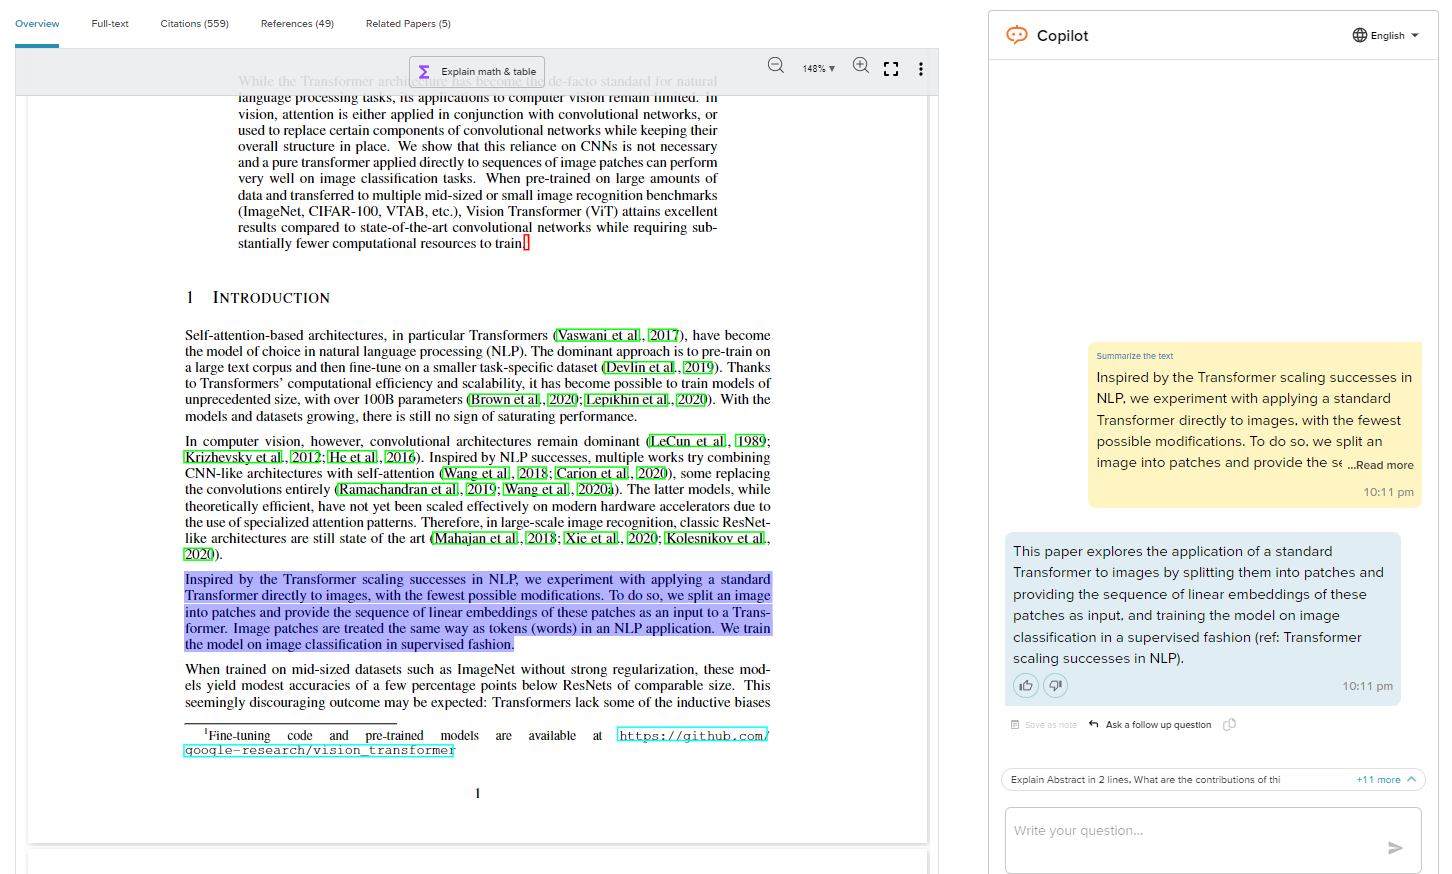
\includegraphics{img/typeset-example.png}
	\caption{Informatie opvragen van een wetenschappelijk artikel met SciSpace}
	\label{img:scispace-example}
\end{figure}

\begin{figure}[H]
	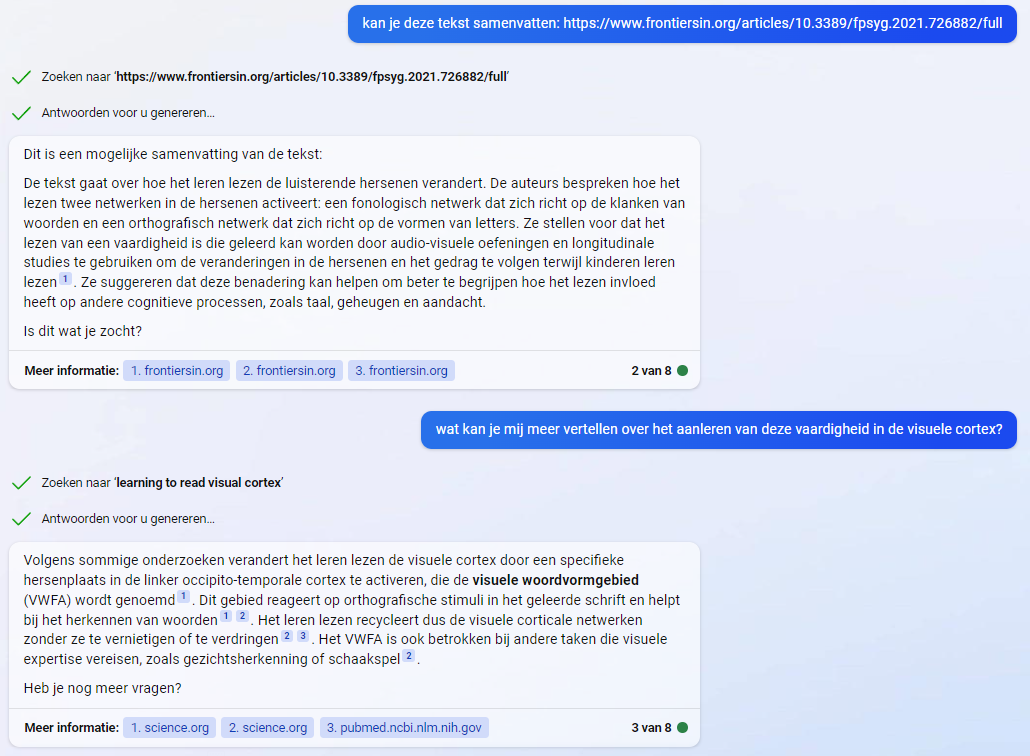
\includegraphics{img/bing-ai-chatbot-example.png}
	\caption{Tekstvereenvoudiging via de link van een wetenschappelijk artikel met Bing Chat}
	\label{img:tryout-bing-ai}
\end{figure}

\begin{figure}[H]
	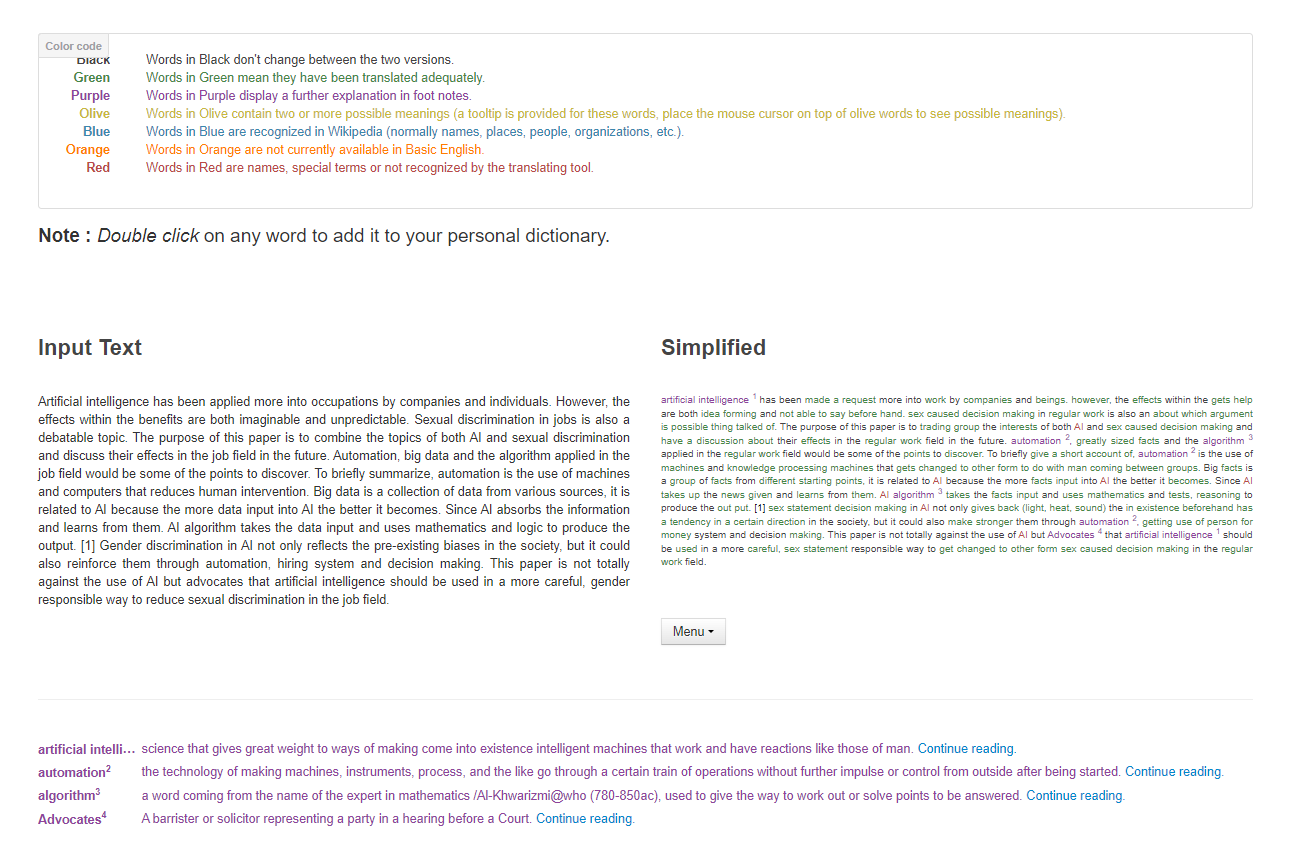
\includegraphics[width=\linewidth]{img/simplish-output.png}
	\caption{Illustratie van de tekstanalyse bij Simplish na een tekstvereenvoudiging.}
	\label{img:simplish-output}
\end{figure}

\begin{figure}[H]
	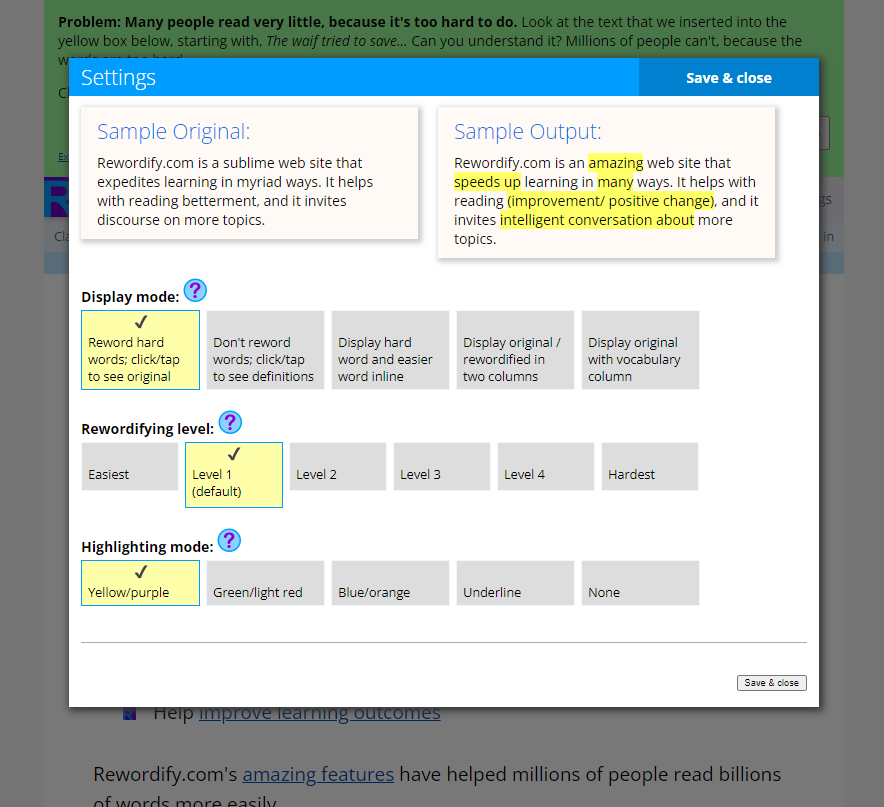
\includegraphics[width=\linewidth]{img/scholarcy-attempt.png}
	\caption{Illustratie van de tekstanalyse bij Rewordify.}
	\label{img:scholarcy}
\end{figure}

\section{Geschikte taalmodel voor gepersonaliseerde tekstvereenvoudiging met ATS}


De vergelijkende studie beoordeelt de uitvoer van de uitgeteste taallmodellen, beschreven in \ref{table:vergelijkende-studie-taalmodellen}, met een subjectieve en een objectieve benadering. Zo achterhaalt deze onderzoeksmethode welk taalmodel of LLM beter aansluit bij het aanbieden van gepersonaliseerde ATS voor scholieren met dyslexie in de derde graad van het middelbaar onderwijs. 

\medspace

Zowel A1 en A2 bevatten meer zinnen na het vereenvoudigen met T1, T2 en T3 vergeleken met de oorspronkelijke tekst, zoals weergegeven in tabel \ref{table:resultaten-aantal-zinnen}. Daarnaast gebruiken T1, T2 en T3 gemiddeld minder woorden per zin dan het oorspronkelijke artikel. Alleen P3 van T4 slaagt erin om gemiddeld minder woorden per zin te gebruiken dan de oorspronkelijke en de referentieteksten van zowel leerlingen en de referentieteksten van leerkrachten, vergeleken met P1 en P2 die elk gemiddeld meer dan 19 woorden per zin gebruiken, zoals te zien is in figuren \ref{img:boxplot-min-max-avg-words-a1} en \ref{img:boxplot-min-max-avg-words-a2}. 

\begin{table}[h]
	\centering
	\begin{tabular}{ | m{3cm} | m{3cm} | m{3cm} | } 
		\hline
		Bron & #Zinnen in A1 & #Zinnen in A2 \\
		\hline
		Oorspronkelijk & 78  & 159 \\ 
		\hline
		MTS (door leerkracht) & 43 & 45 \\
		\hline
		MTS (door leerling) & n.v.t. & 50 \\
		\hline
		T1 & 101 & 209 \\
		\hline
		T2 & 82 & 209 \\
		\hline
		T3 & 100 & 209 \\
		\hline
		T4 P1 & 61 & 98 \\
		\hline
		T4 P2 & 89 & 133 \\
		\hline
		T4 P3 & 39 & 55 \\
		\hline
	\end{tabular}
	\label{table:resultaten-aantal-zinnen}
	\caption{Aantal zinnen (gemeten met Spacy sentence embeddings) per tekst.}
\end{table}

\begin{figure}
	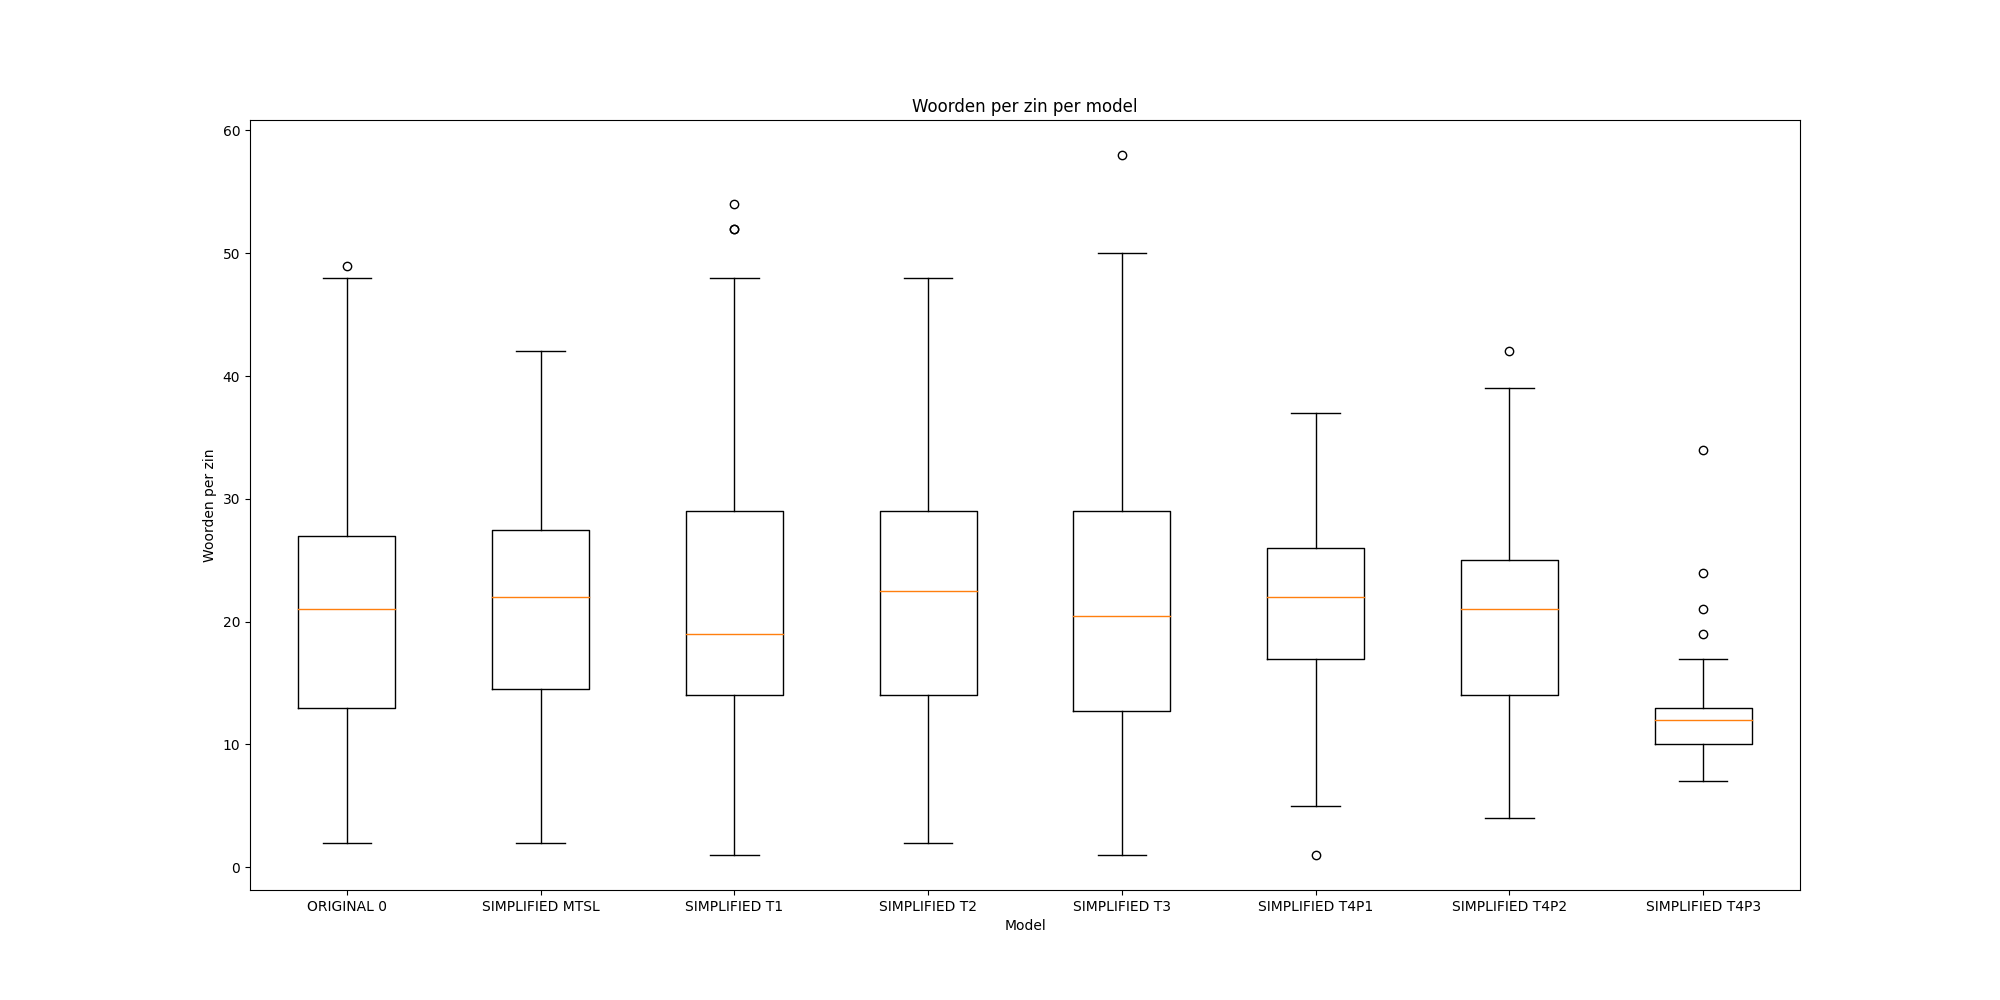
\includegraphics[width=\linewidth]{img/boxplot-avg-a1.png}
	\caption{Overzicht van het minimum, maximum en gemiddeld aantal woorden per zin per model in A1.}
	\label{img:boxplot-min-max-avg-words-a1}
\end{figure}

\begin{figure}
	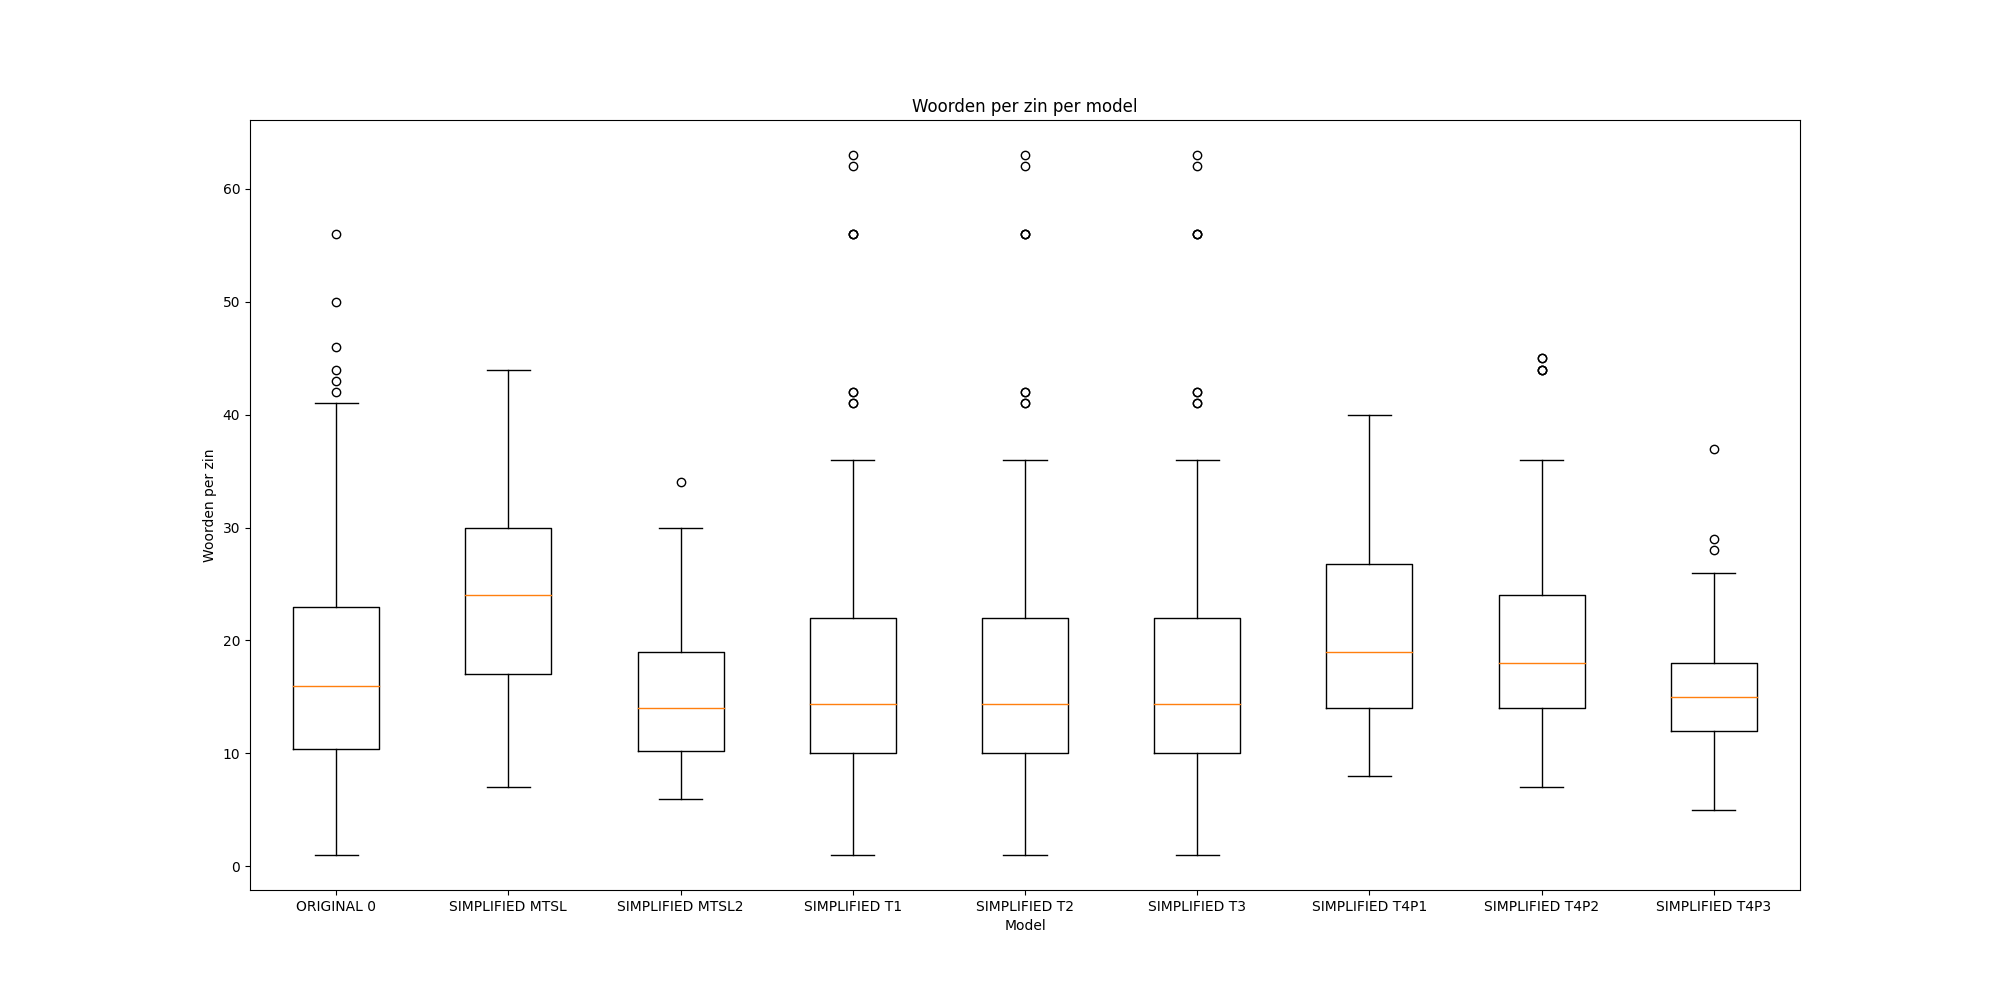
\includegraphics[width=\linewidth]{img/boxplot-avg-a2.png}
	\caption{Overzicht van het minimum, maximum en gemiddeld aantal woorden per zin per model in A2.}
	\label{img:boxplot-min-max-avg-words-a2}
\end{figure}

De FRE-scores van alle geteste taalmodellen en MTS-referentieteksten zijn niet significant hoger of lager dan die van het oorspronkelijke wetenschappelijke artikel, zoals weergegeven in figuren \ref{img:boxplot-fre-a1} en \ref{img:boxplot-fre-a2}. Evenzo zijn de FOG-scores ook niet significant hoger of lager bij de vereenvoudigde wetenschappelijke artikelen, zoals aangegeven in figuren \ref{img:boxplot-fog-a1} en \ref{img:boxplot-fog-a2}. 


\begin{figure}
	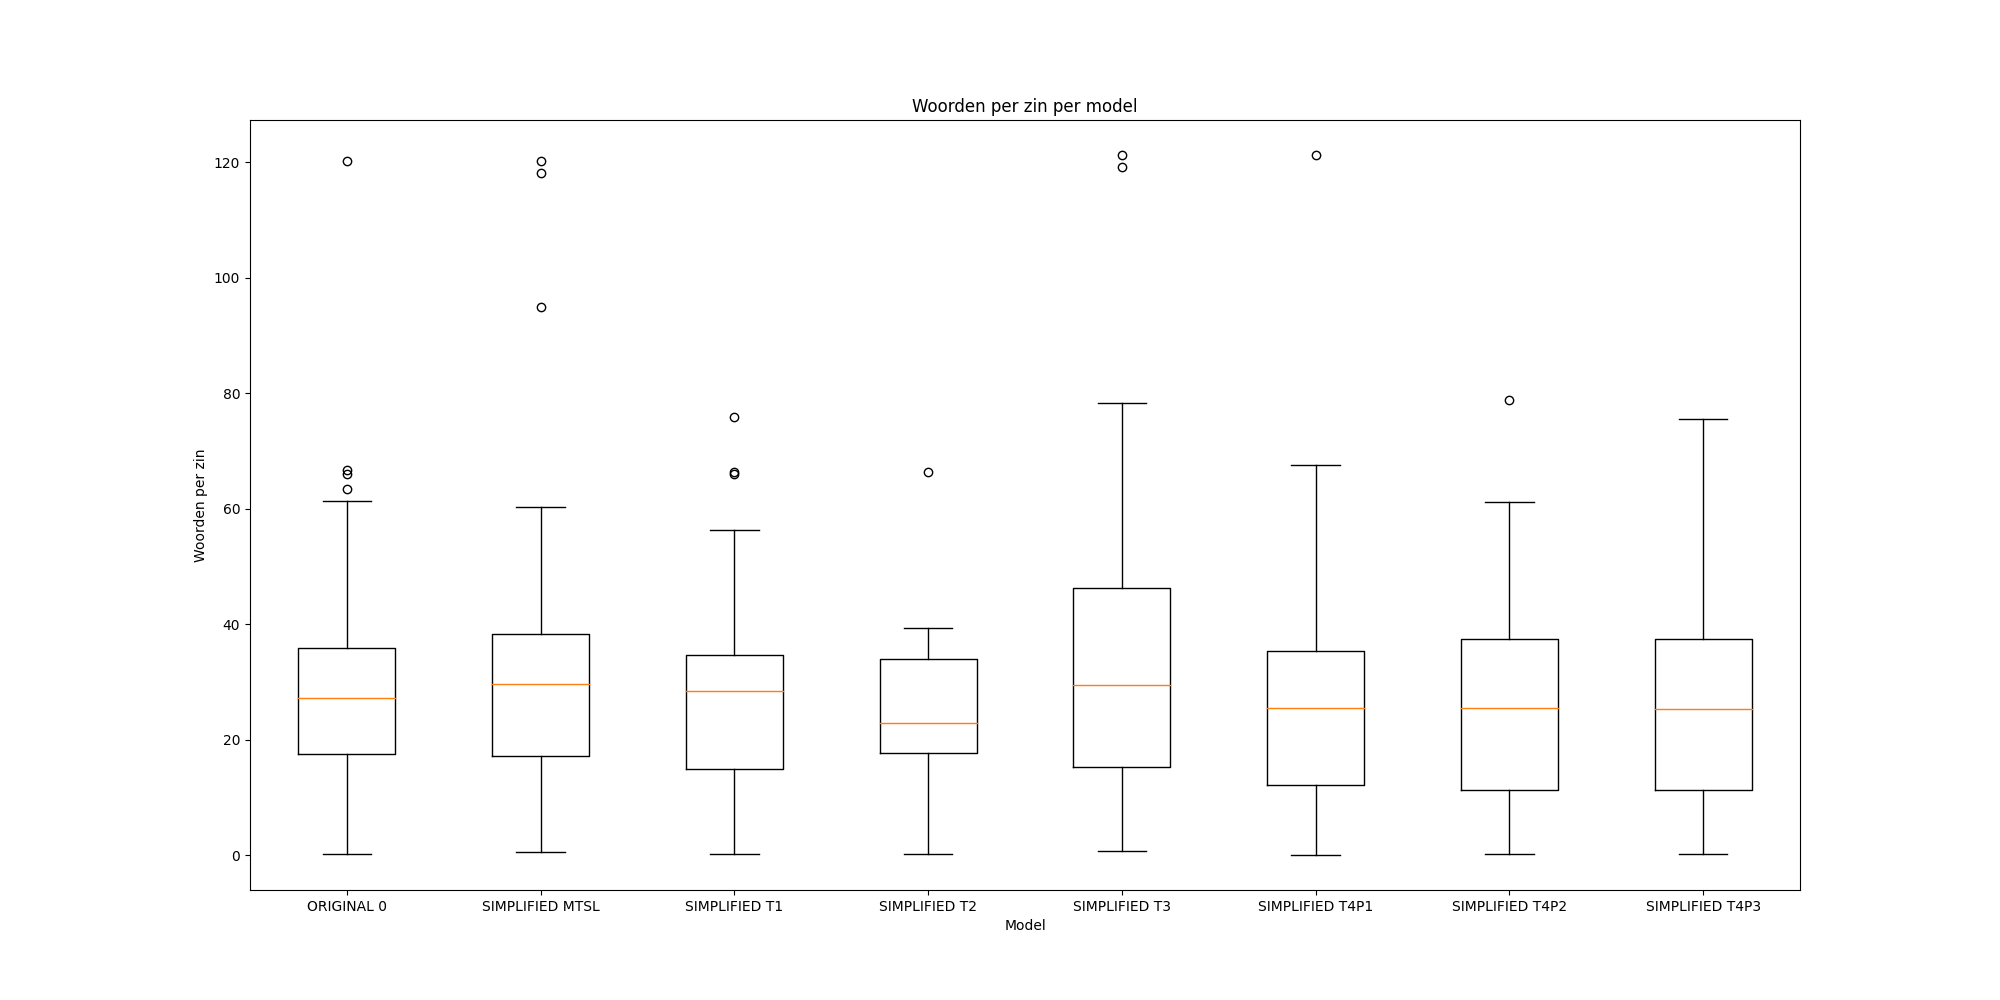
\includegraphics[width=\linewidth]{img/boxplot-fre-a1.png}
	\caption{Boxplot van de FRE-scores voor A1.}
	\label{img:boxplot-fre-a1}
\end{figure}

\begin{figure}
	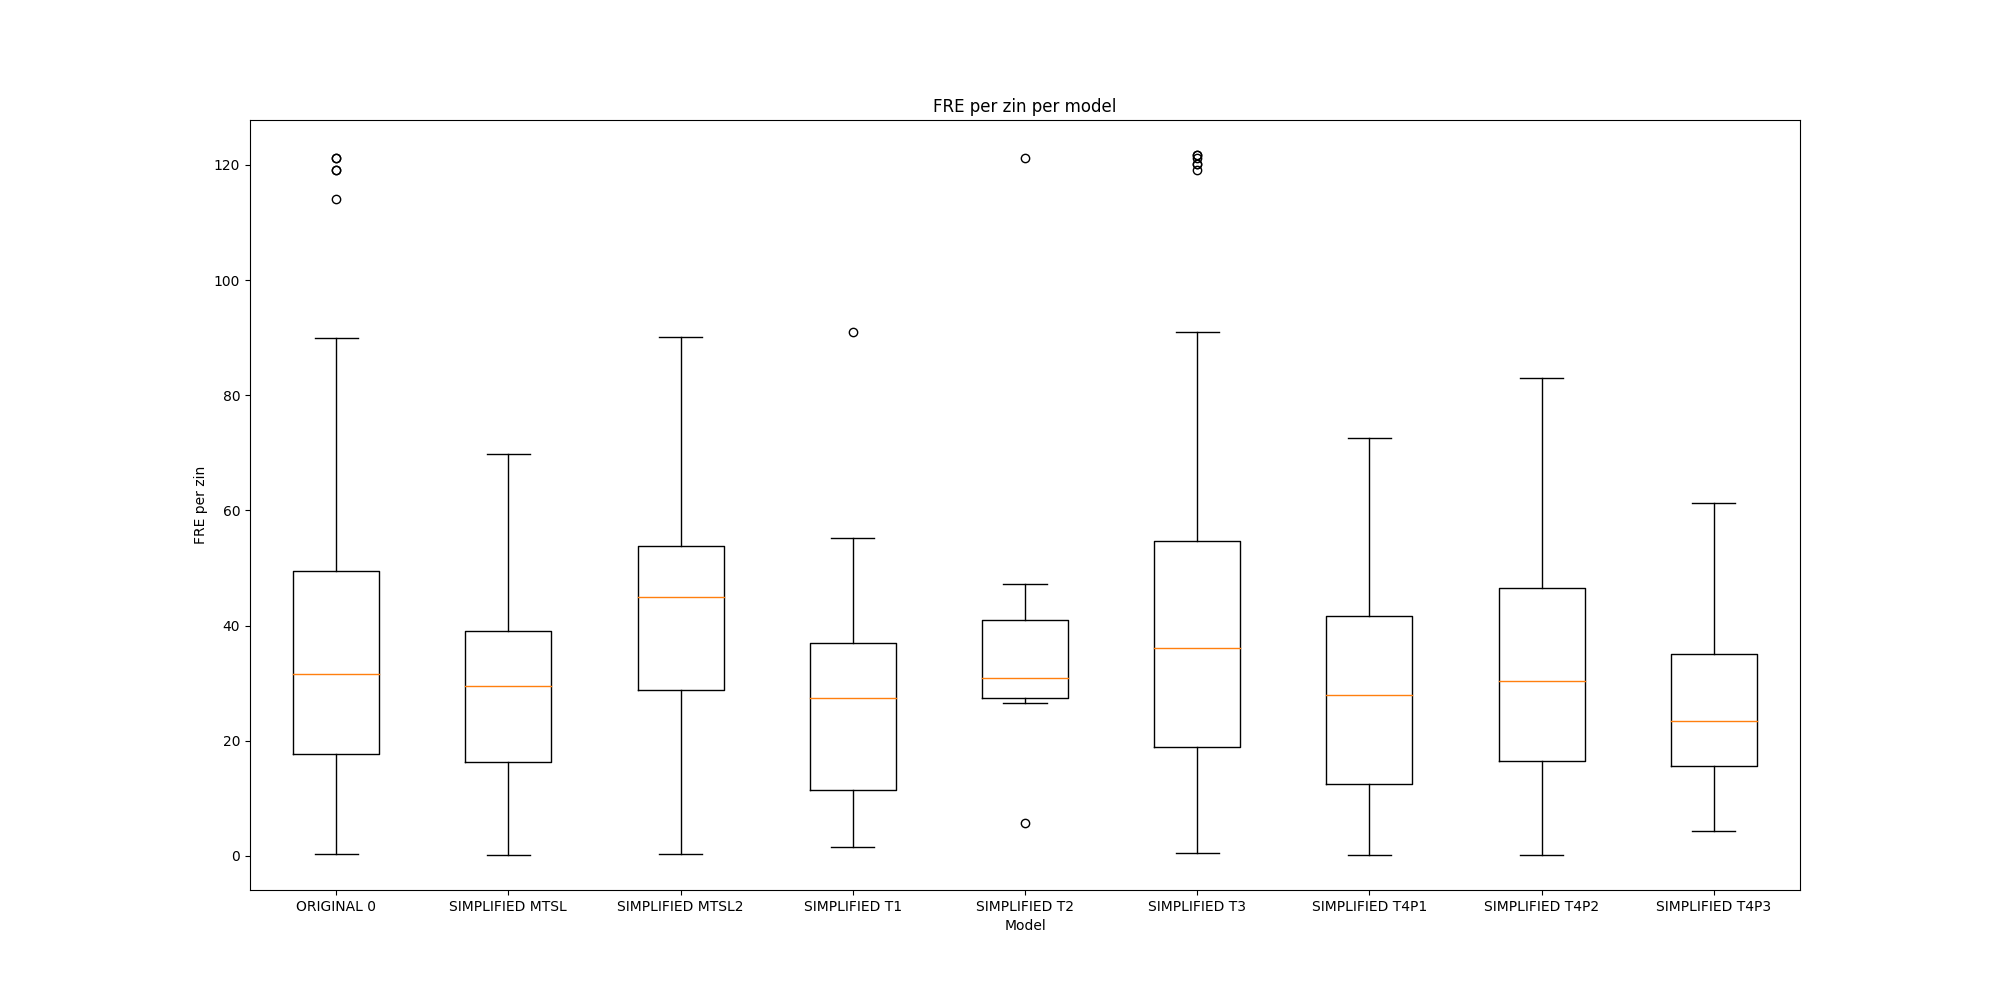
\includegraphics[width=\linewidth]{img/boxplot-fre-a2.png}
	\caption{Boxplot van de FRE-scores voor A2.}
	\label{img:boxplot-fre-a2}
\end{figure}

\begin{figure}
	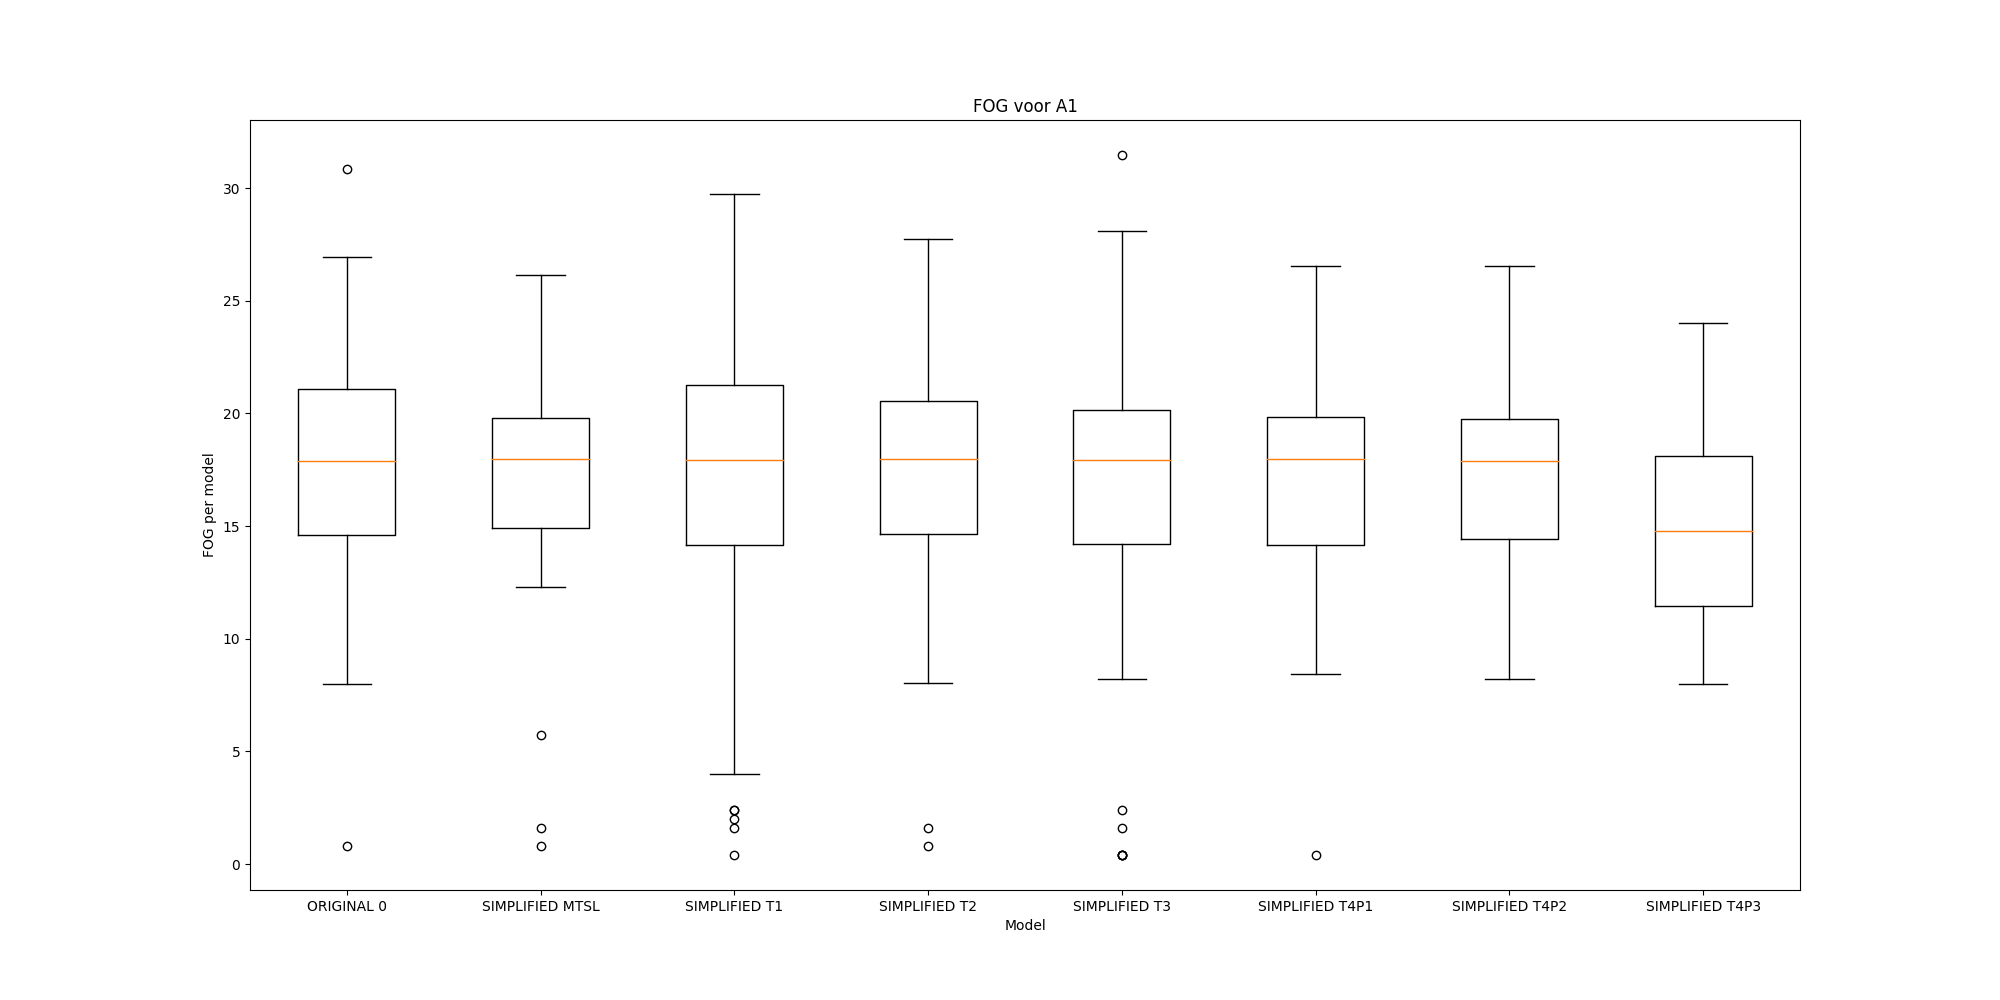
\includegraphics[width=\linewidth]{img/boxplot-fog-a1.png}
	\caption{Boxplot van de FOG-scores voor A1.}
	\label{img:boxplot-fog-a1}
\end{figure}

\begin{figure}
	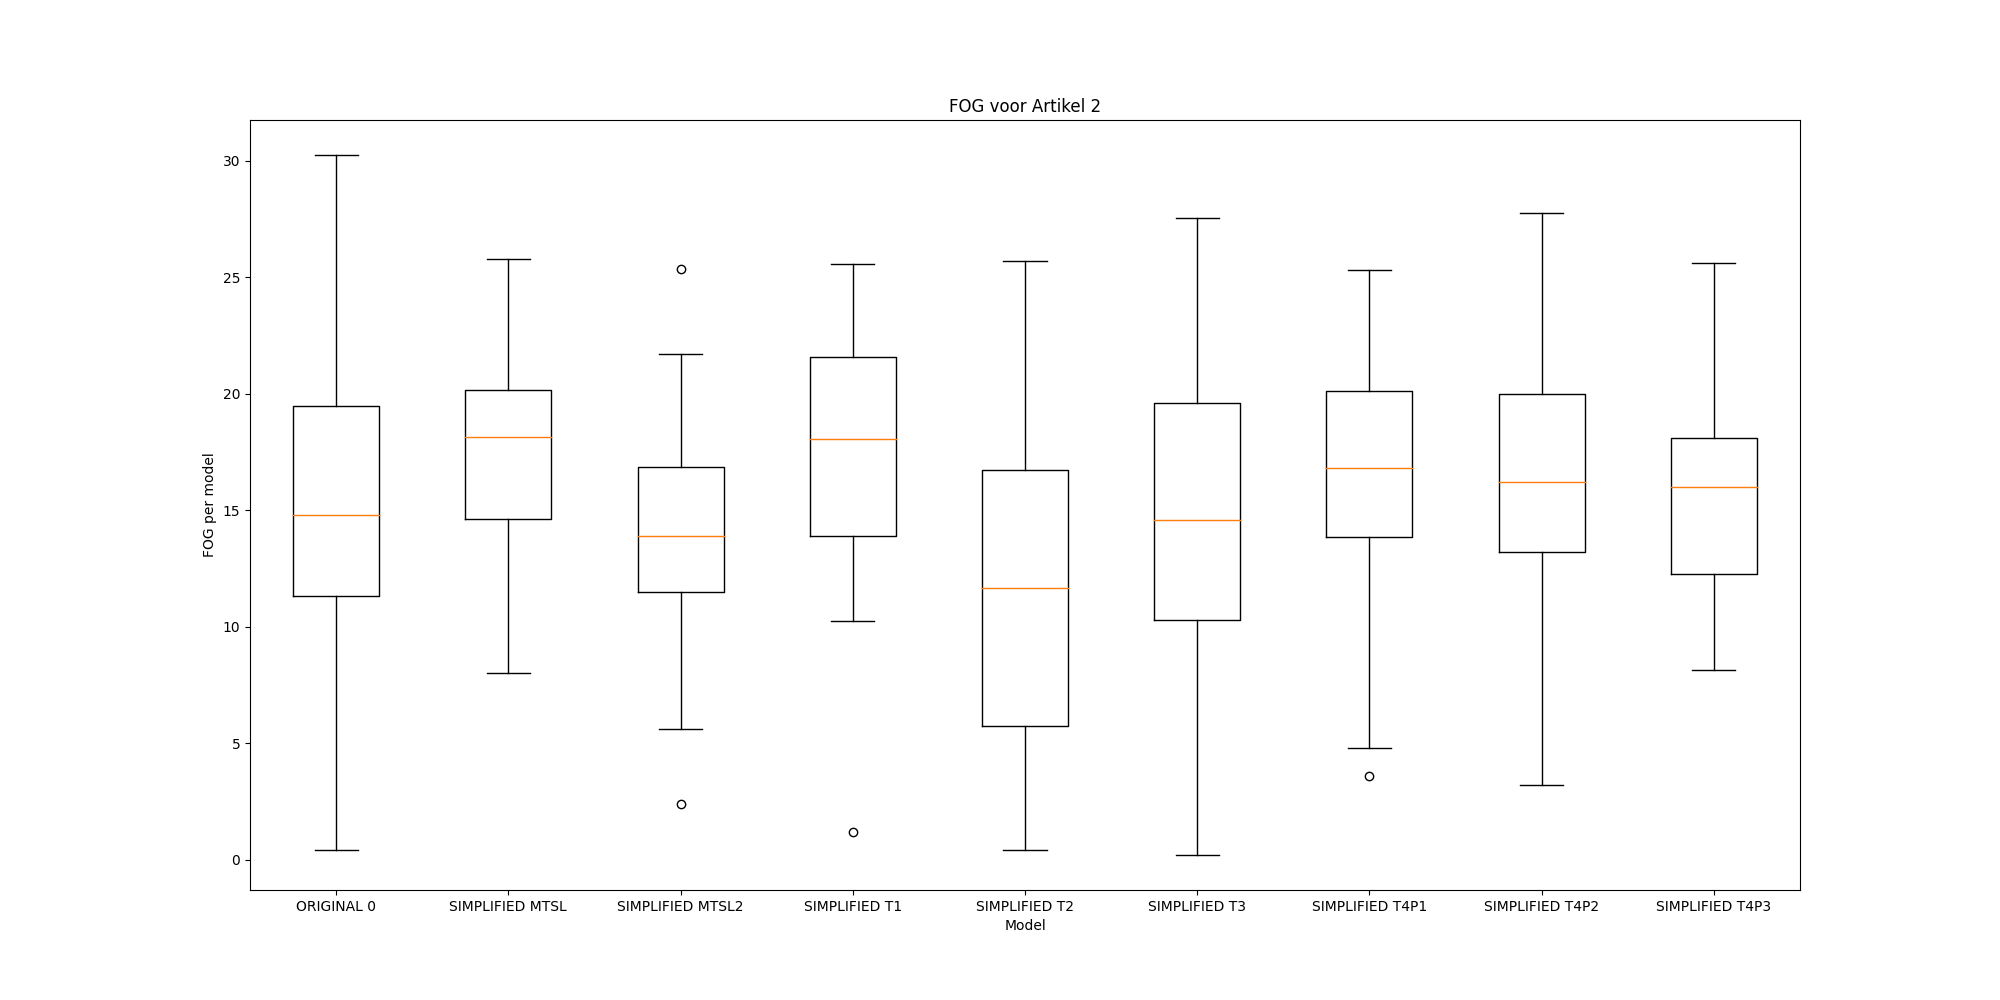
\includegraphics[width=\linewidth]{img/boxplot-fog-a2.png}
	\caption{Boxplot van de FOG-scores voor A2.}
	\label{img:boxplot-fog-a2}
\end{figure}

T1, T2 en T3 gebruiken bij zowel A1 als A2 langere woorden vergeleken met de oorspronkelijke tekst, in tegenstelling tot alle T4 prompts die wel langere woorden wegwerken en zo een gelijk resultaat bekomen als de MTS referentieteksten. Deze verhouding wordt aangewezen in figuur \ref{img:violinplot-long-a1} en figuur \ref{img:violinplot-long-a2}. Daarnaast vervangen T1, T2 en T3 ook minder complexe woorden vergeleken met T4 en de MTS-referentietekst. Dit verschil wordt geïllustreerd in figuur \ref{img:violinplot-complex-a1} en figuur \ref{img:violinplot-complex-a2}.

\begin{figure}
	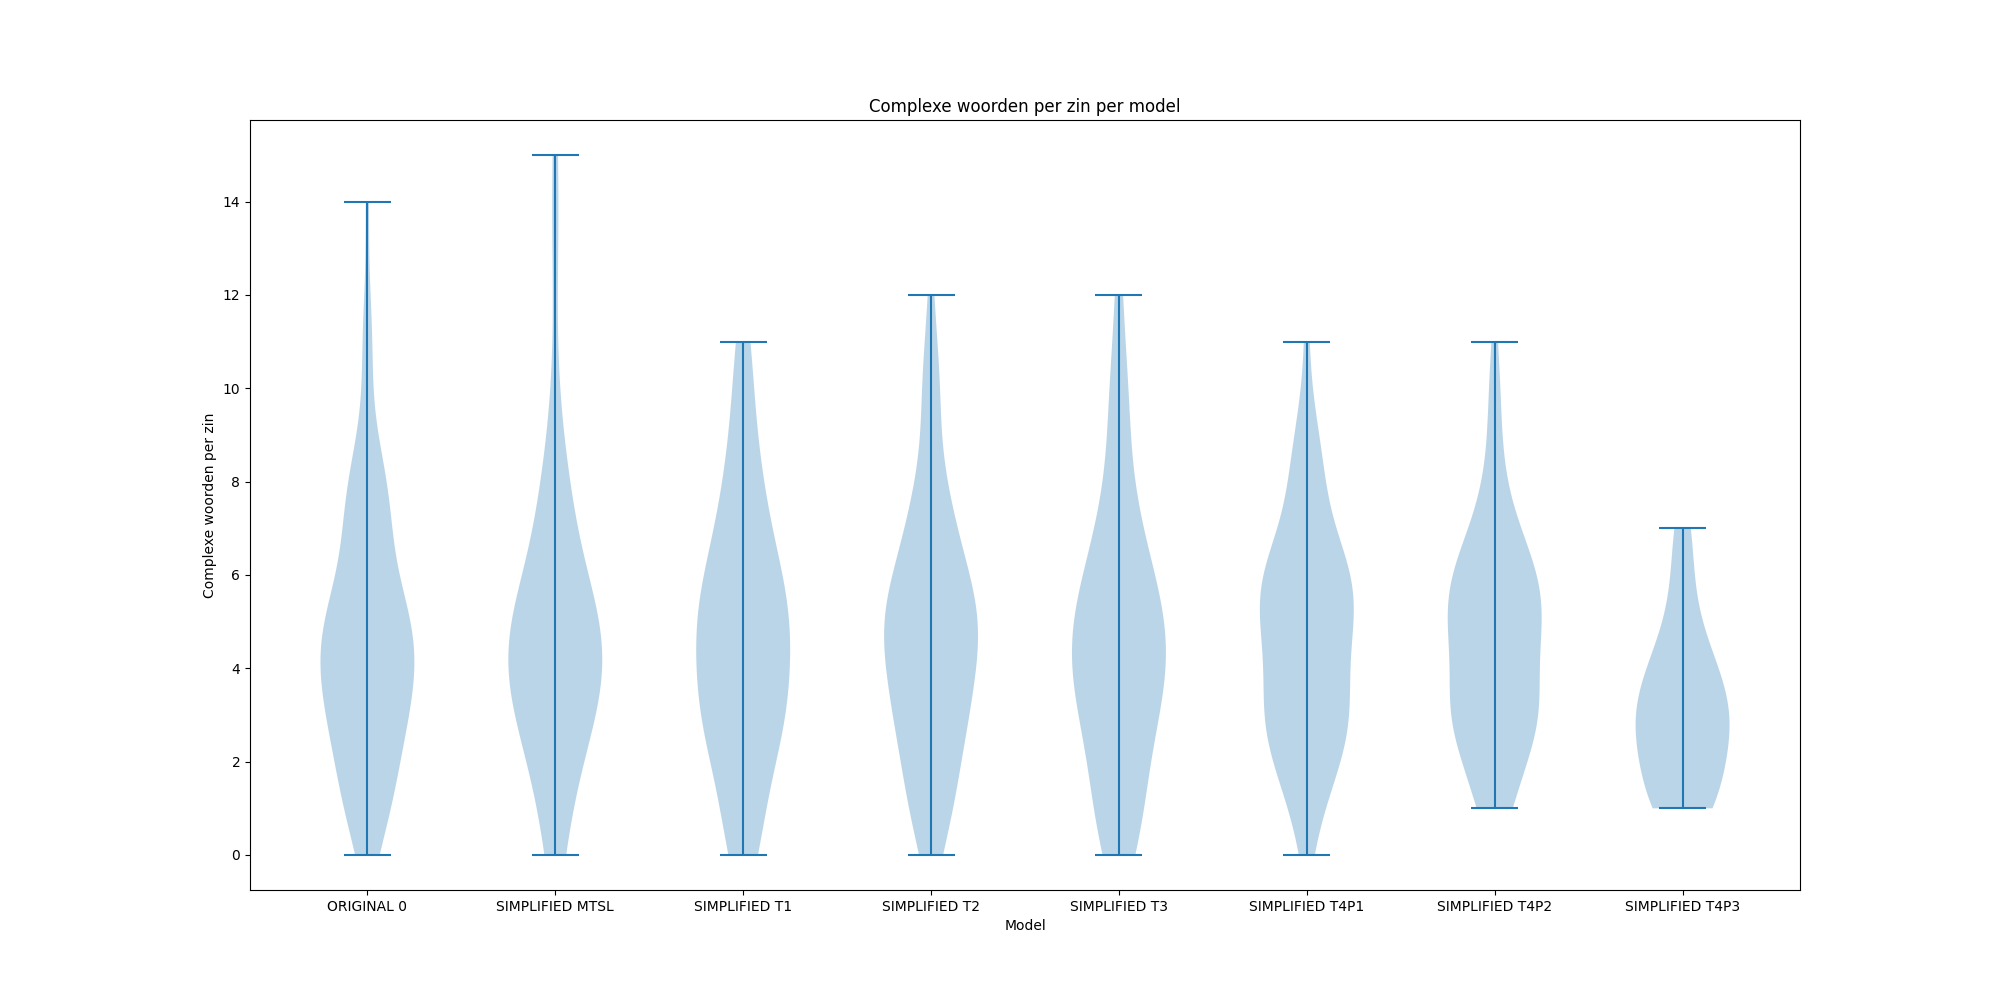
\includegraphics[width=\linewidth]{img/violinplot-complex-a1.png}
	\caption{Gemiddeld aantal complexe woorden per zin gegroepeerd op model voor A1.}
	\label{img:violinplot-complex-a1}
\end{figure}

\begin{figure}
	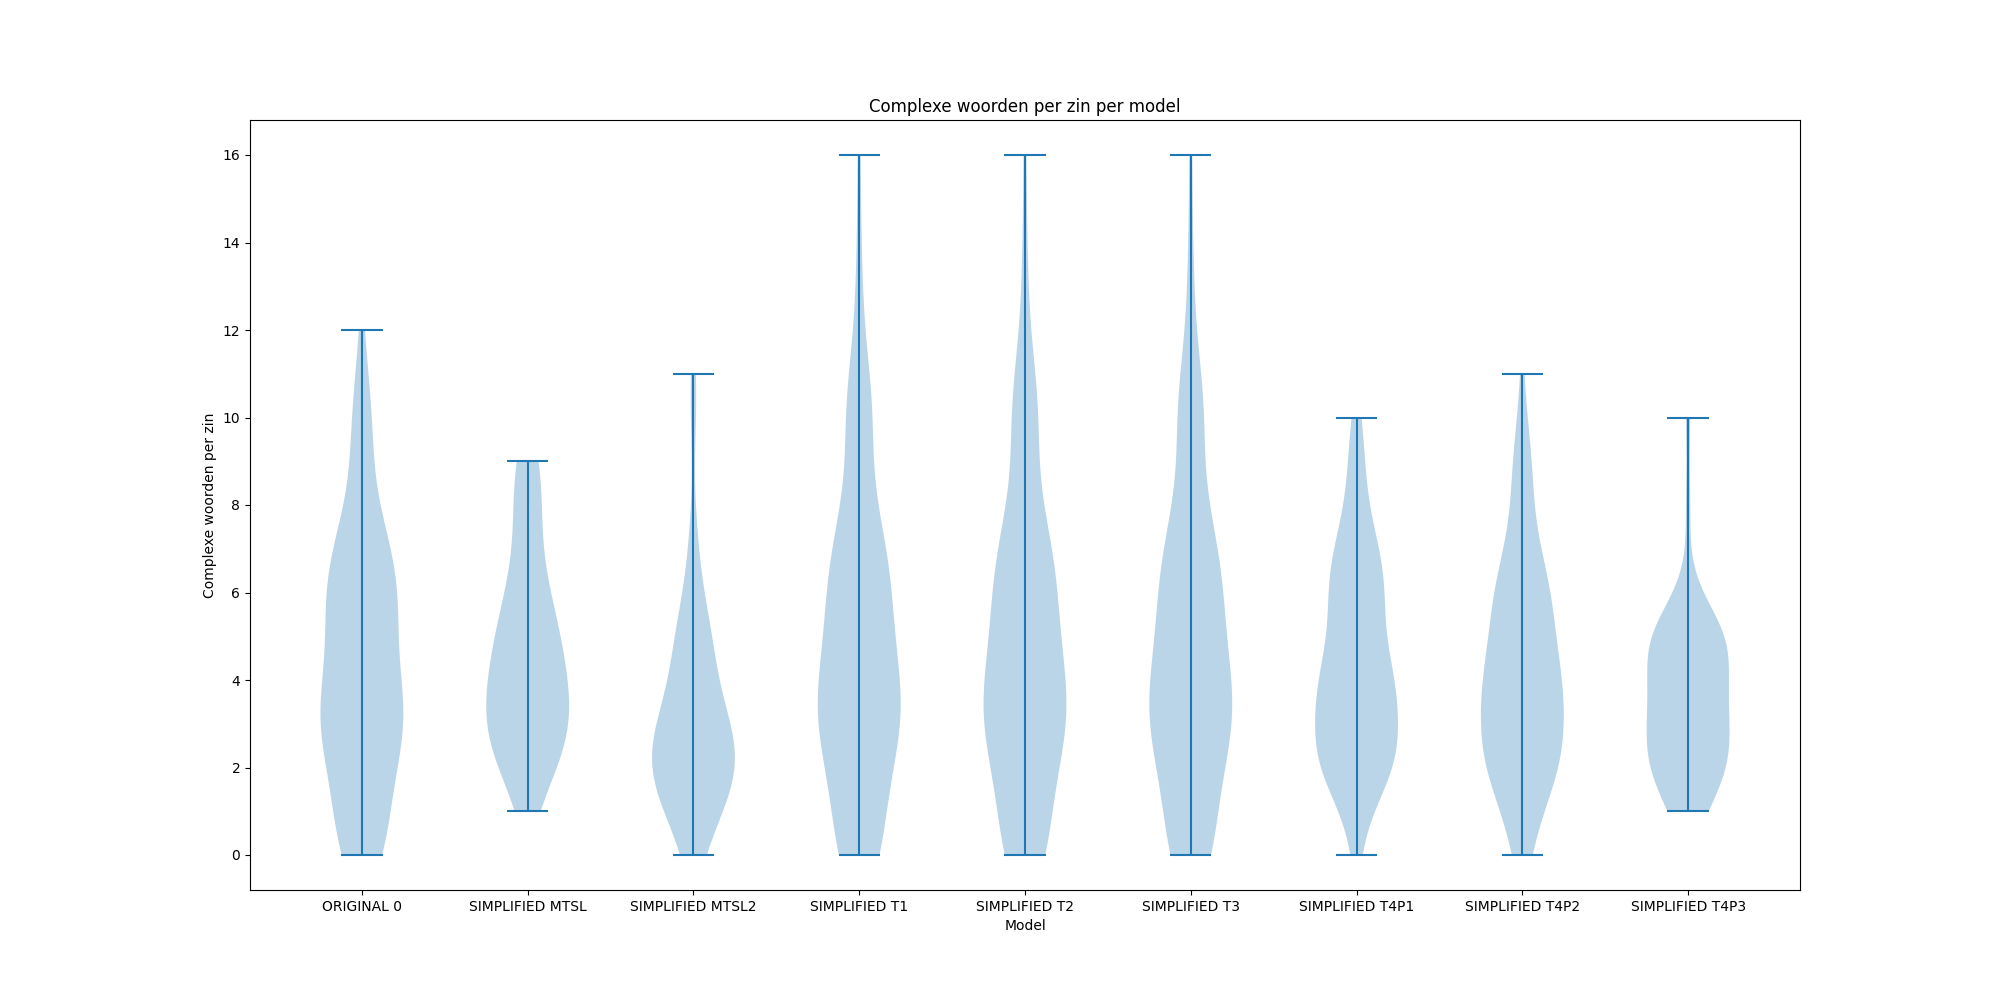
\includegraphics[width=\linewidth]{img/violinplot-complex-a2.png}
	\caption{Gemiddeld aantal complexe woorden per zin gegroepeerd op model voor A2.}
	\label{img:violinplot-complex-a2}
\end{figure}

\begin{figure}
	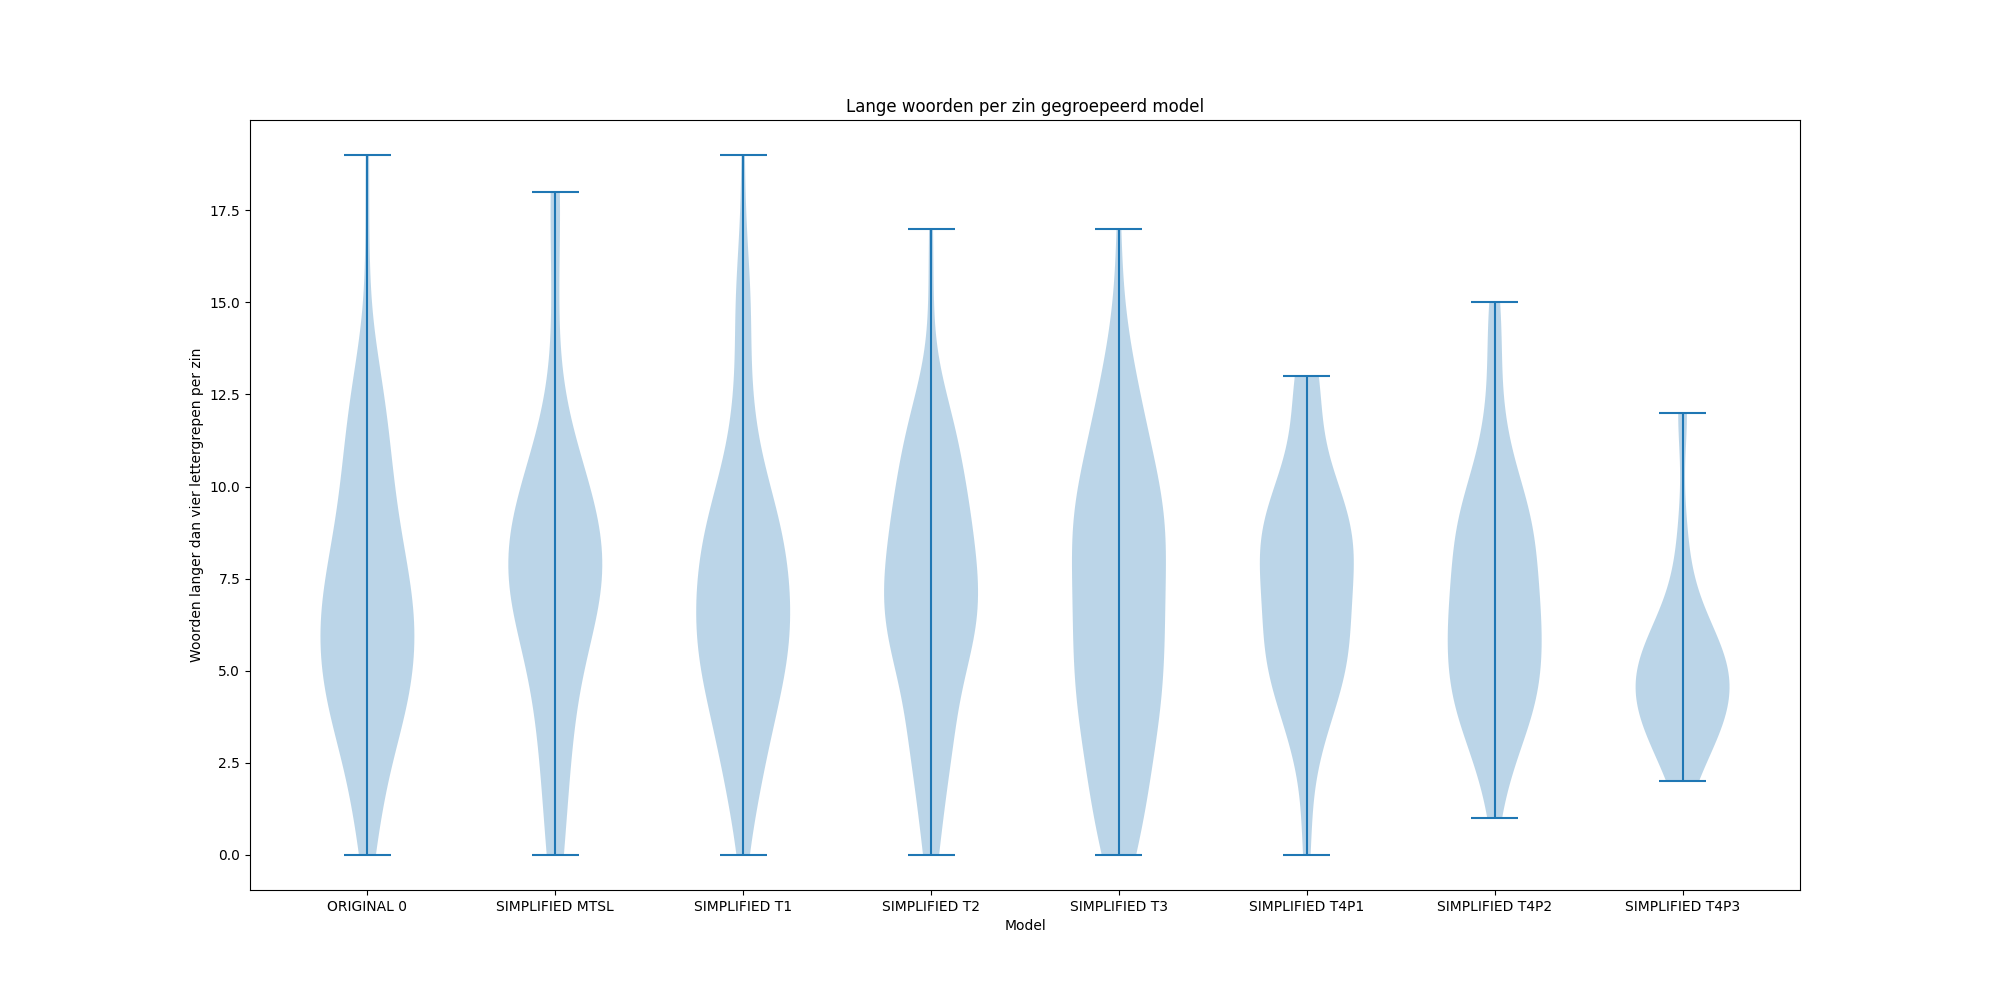
\includegraphics[width=\linewidth]{img/violinplot-long-a1.png}
	\caption{Gemiddeld aantal lange woorden per zin gegroepeerd op model voor A1.}
	\label{img:violinplot-long-a1}
\end{figure}

\begin{figure}
	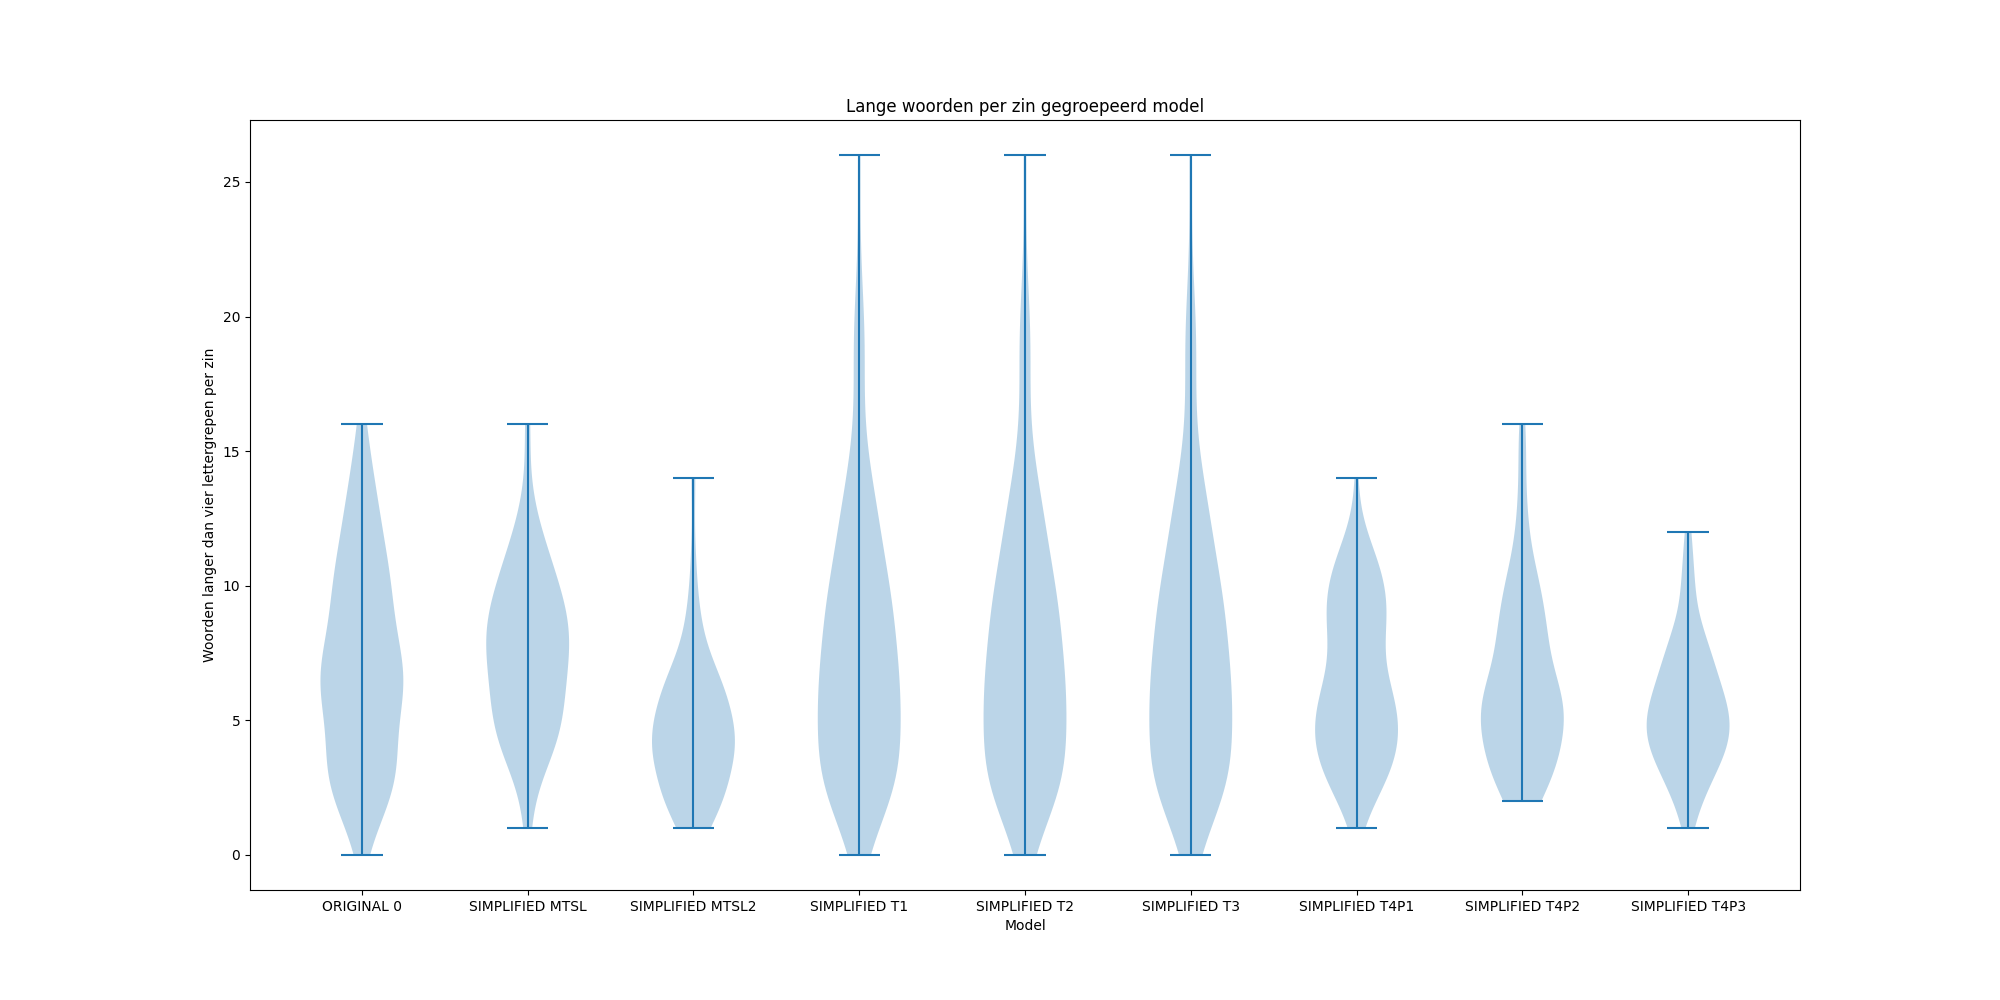
\includegraphics[width=\linewidth]{img/violinplot-long-a2.png}
	\caption{Gemiddeld aantal lange woorden per zin gegroepeerd op model voor A2.}
	\label{img:violinplot-long-a2}
\end{figure}

Ten slotte gebruiken T1, T2 en T3 minder hulpwerkwoorden en vervoegingen van het werkwoord 'zijn'. Daarnaast tonen \ref{img:histplot-aux-a1} en \ref{img:histplot-aux-a2} aan dat alle prompts van T4 een gelijke trend volgen met het aantal vervoegingen en hulpwerkwoorden vergeleken met de MTS-referentieteksten.

\begin{figure}
	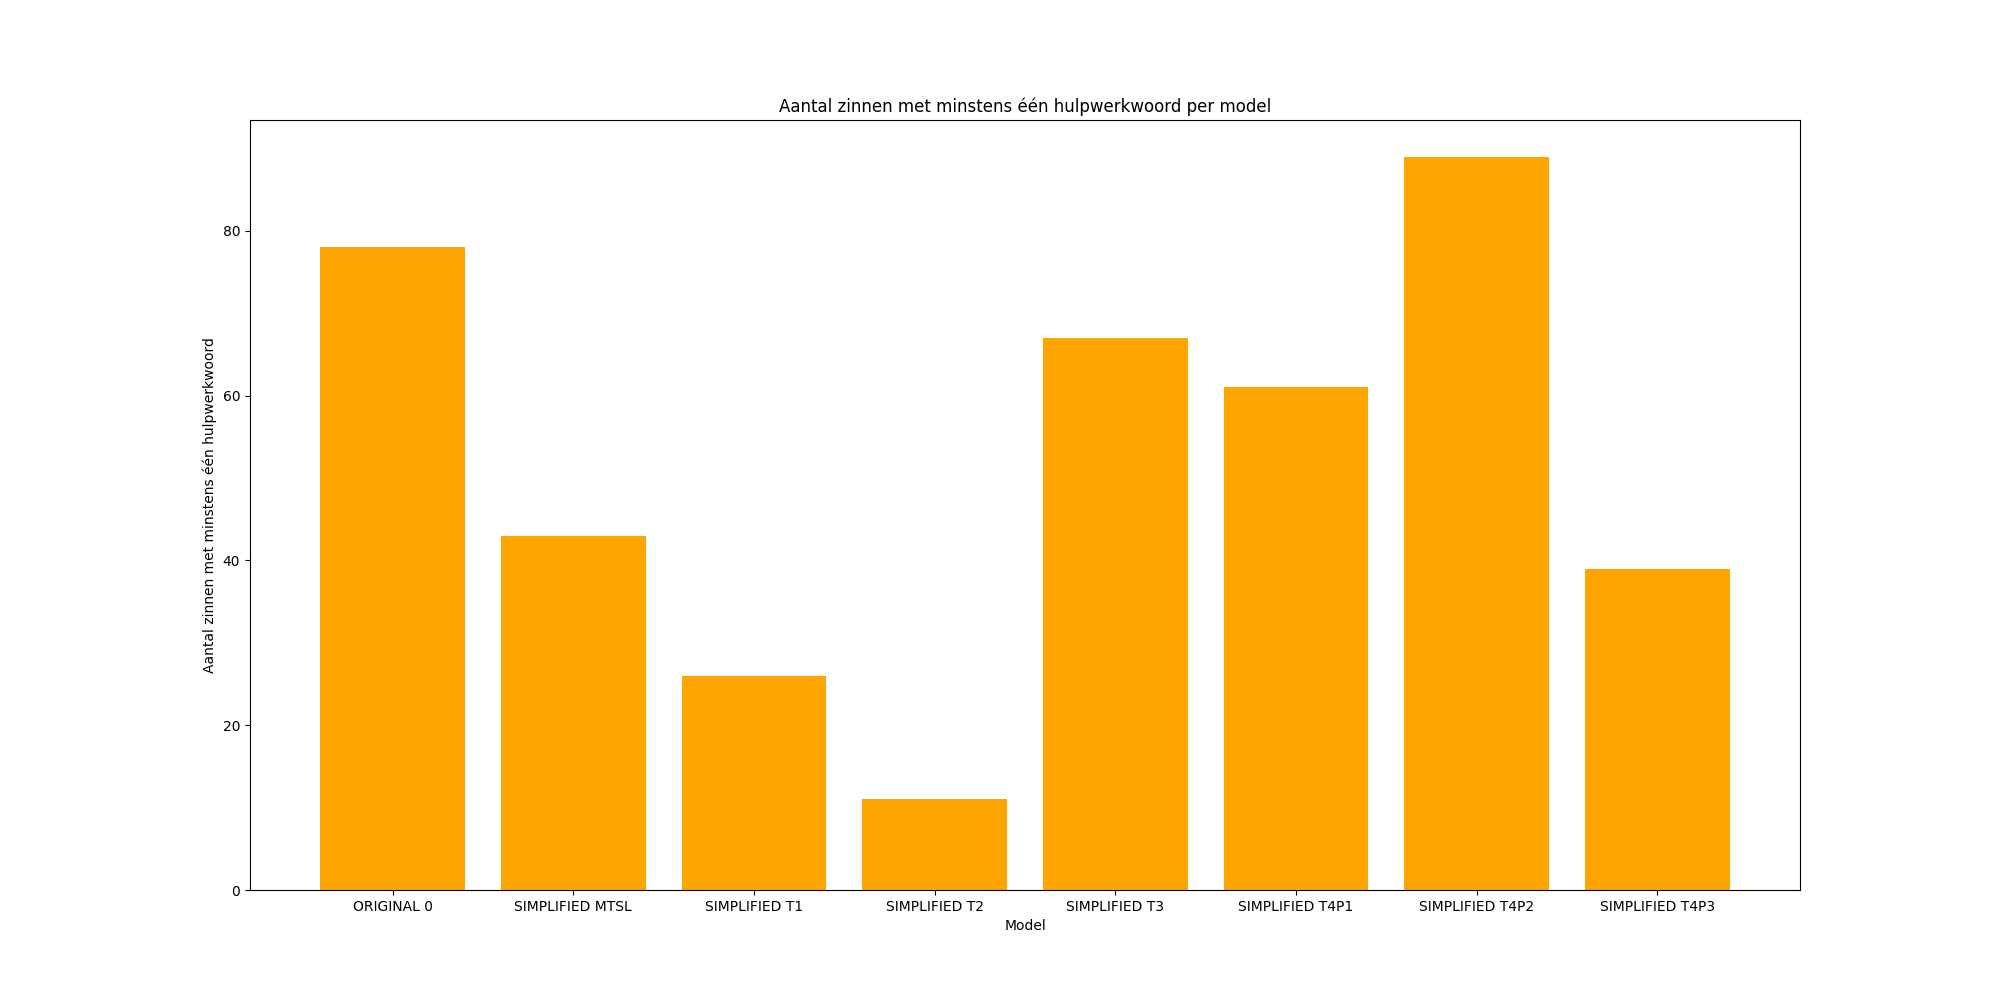
\includegraphics[width=\linewidth]{img/boxplot-aux-a1.png}
	\caption{Gemiddeld aantal hulpwerkwoorden per zin gegroepeerd op model voor A1.}
	\label{img:histplot-aux-a1}
\end{figure}

\begin{figure}
	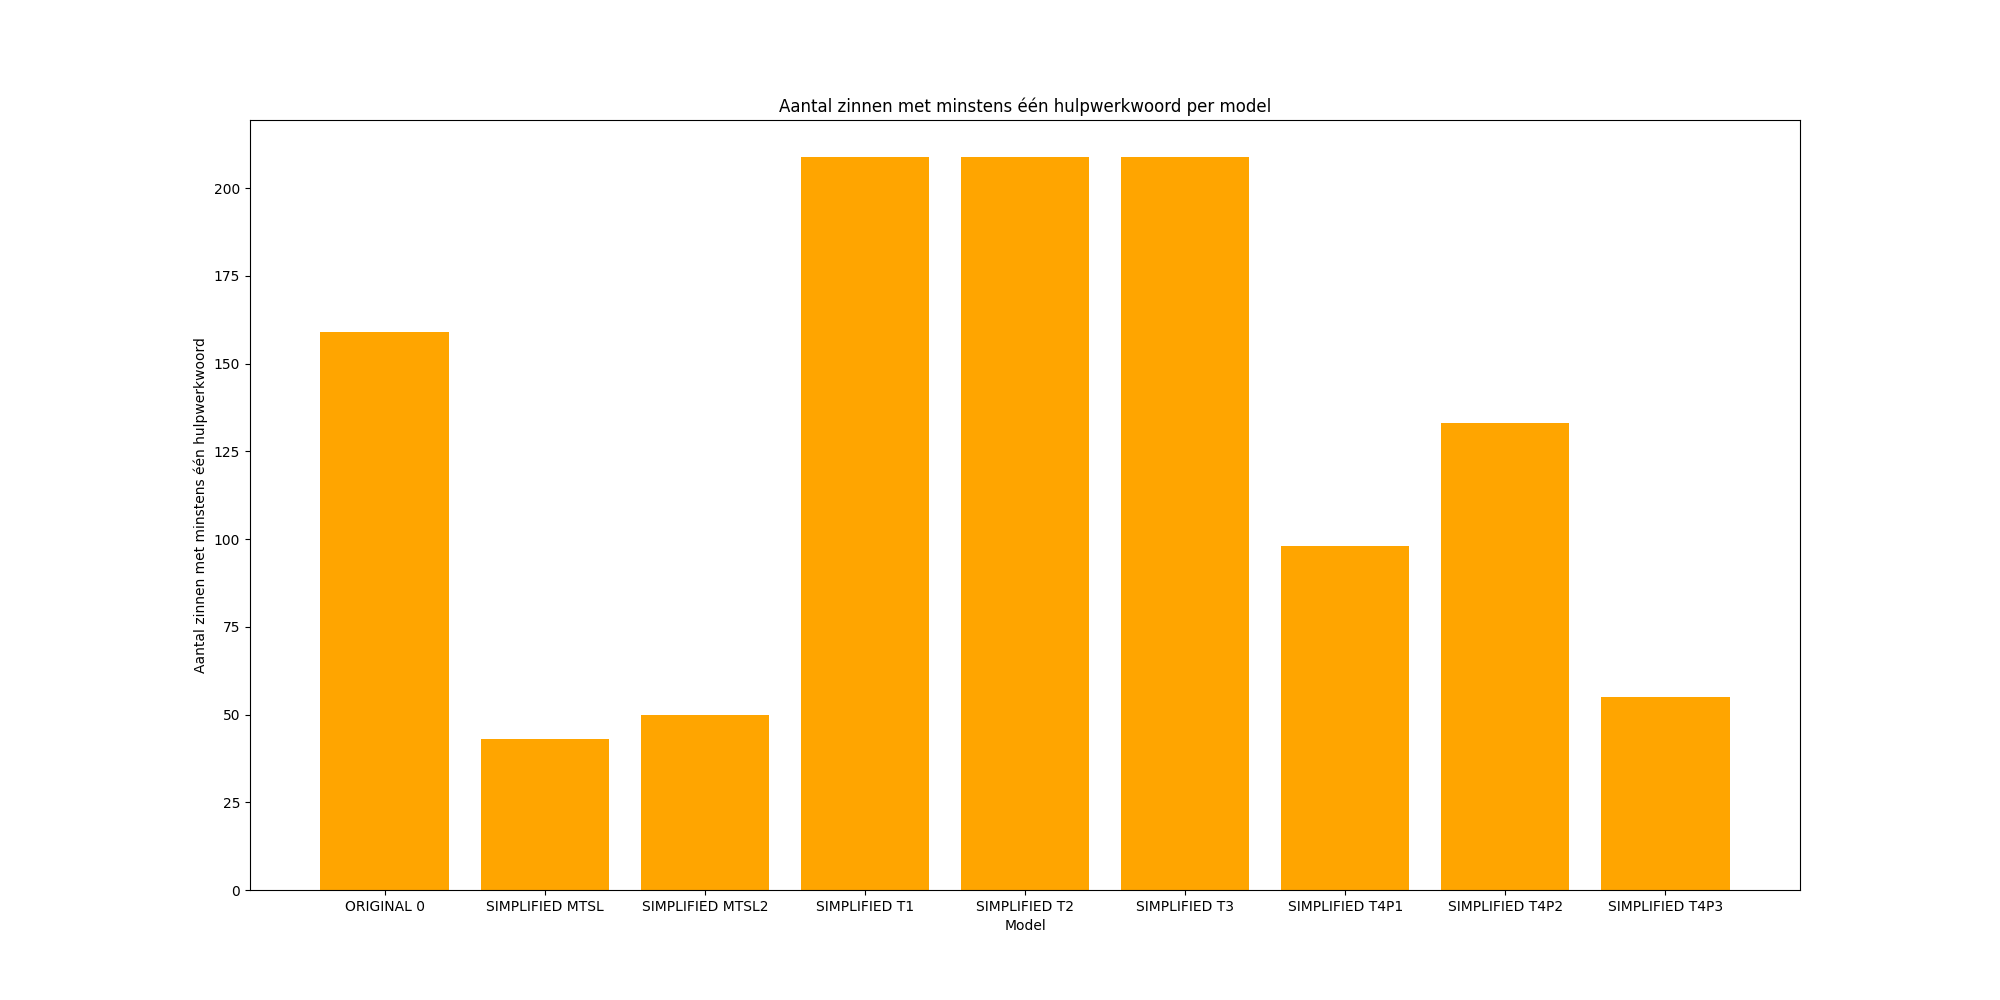
\includegraphics[width=\linewidth]{img/boxplot-aux-a2.png}
	\caption{Gemiddeld aantal hulpwerkwoorden per zin gegroepeerd op model voor A2.}
	\label{img:histplot-aux-a2}
\end{figure}

\begin{figure}
	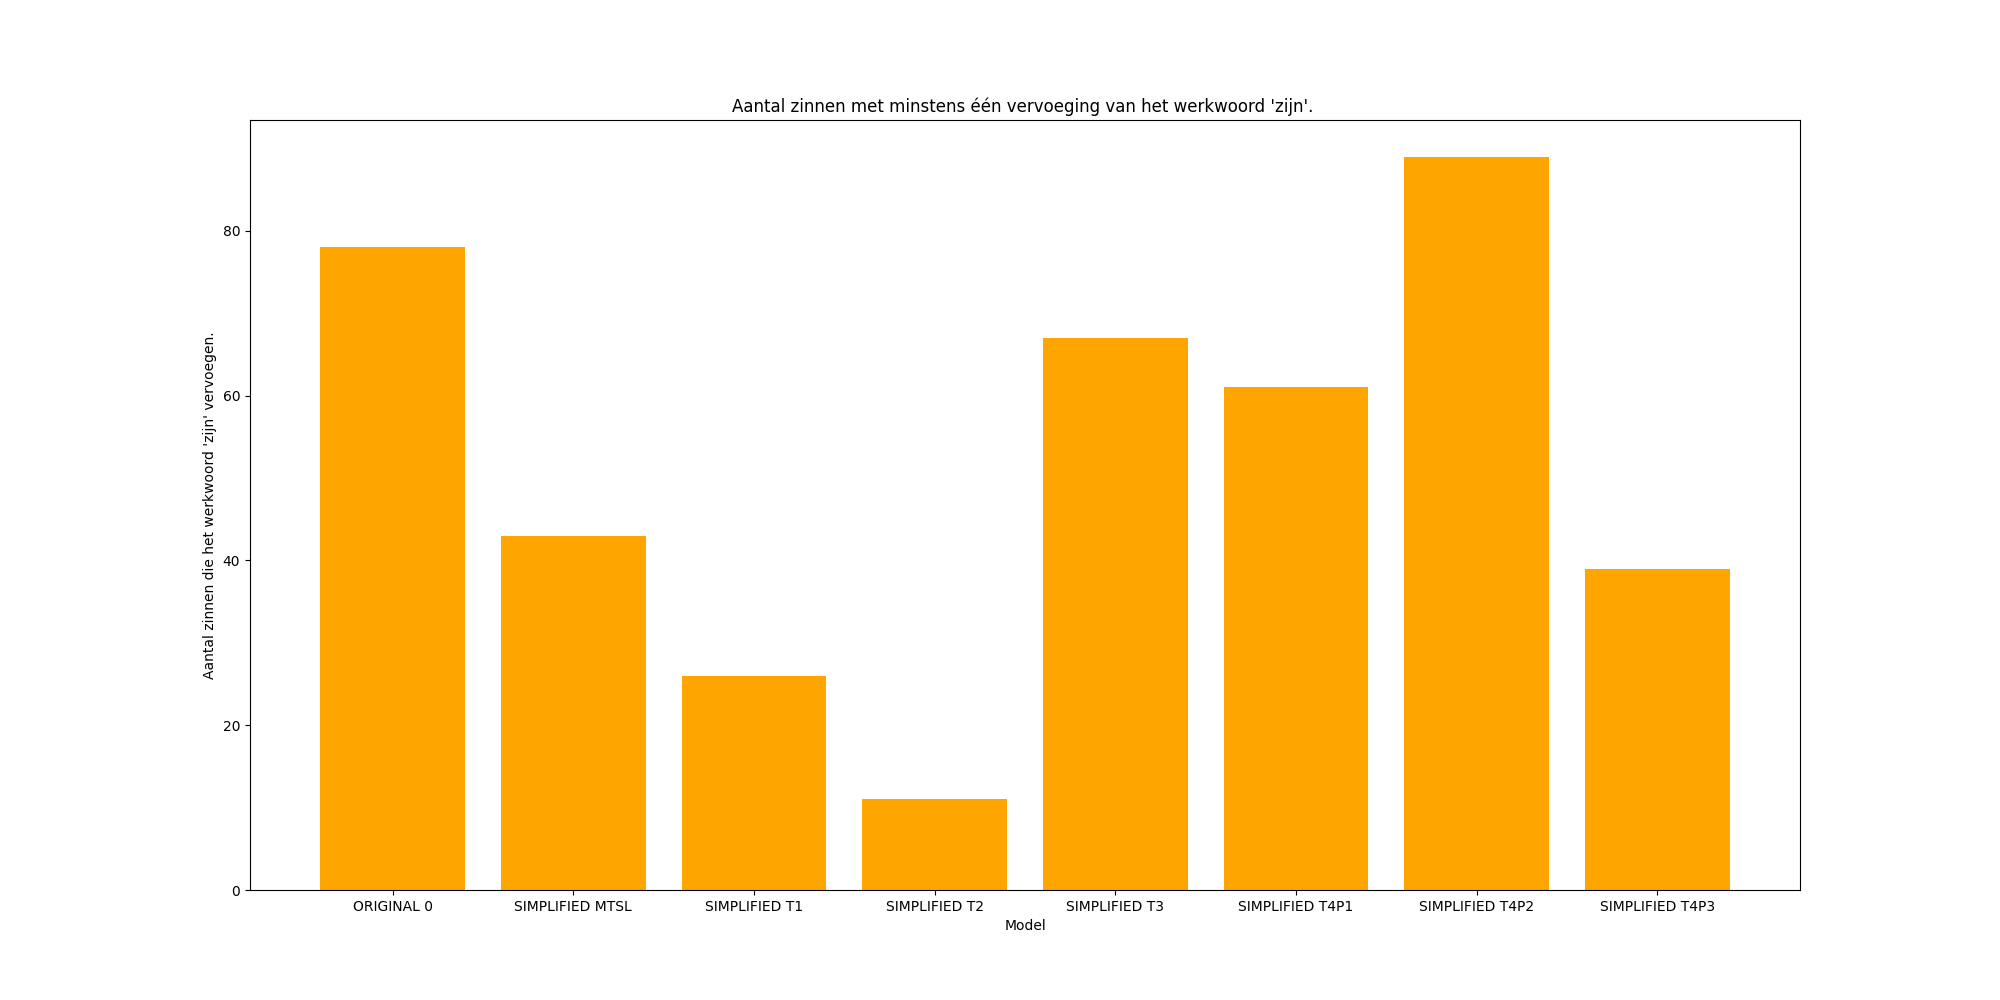
\includegraphics[width=\linewidth]{img/boxplot-tobe-a1.png}
	\caption{Gemiddeld aantal vervoegingen van het werkwoord 'zijn' per zin gegroepeerd op model voor A1.}
	\label{img:histplot-tobe-a1}
\end{figure}

\begin{figure}
	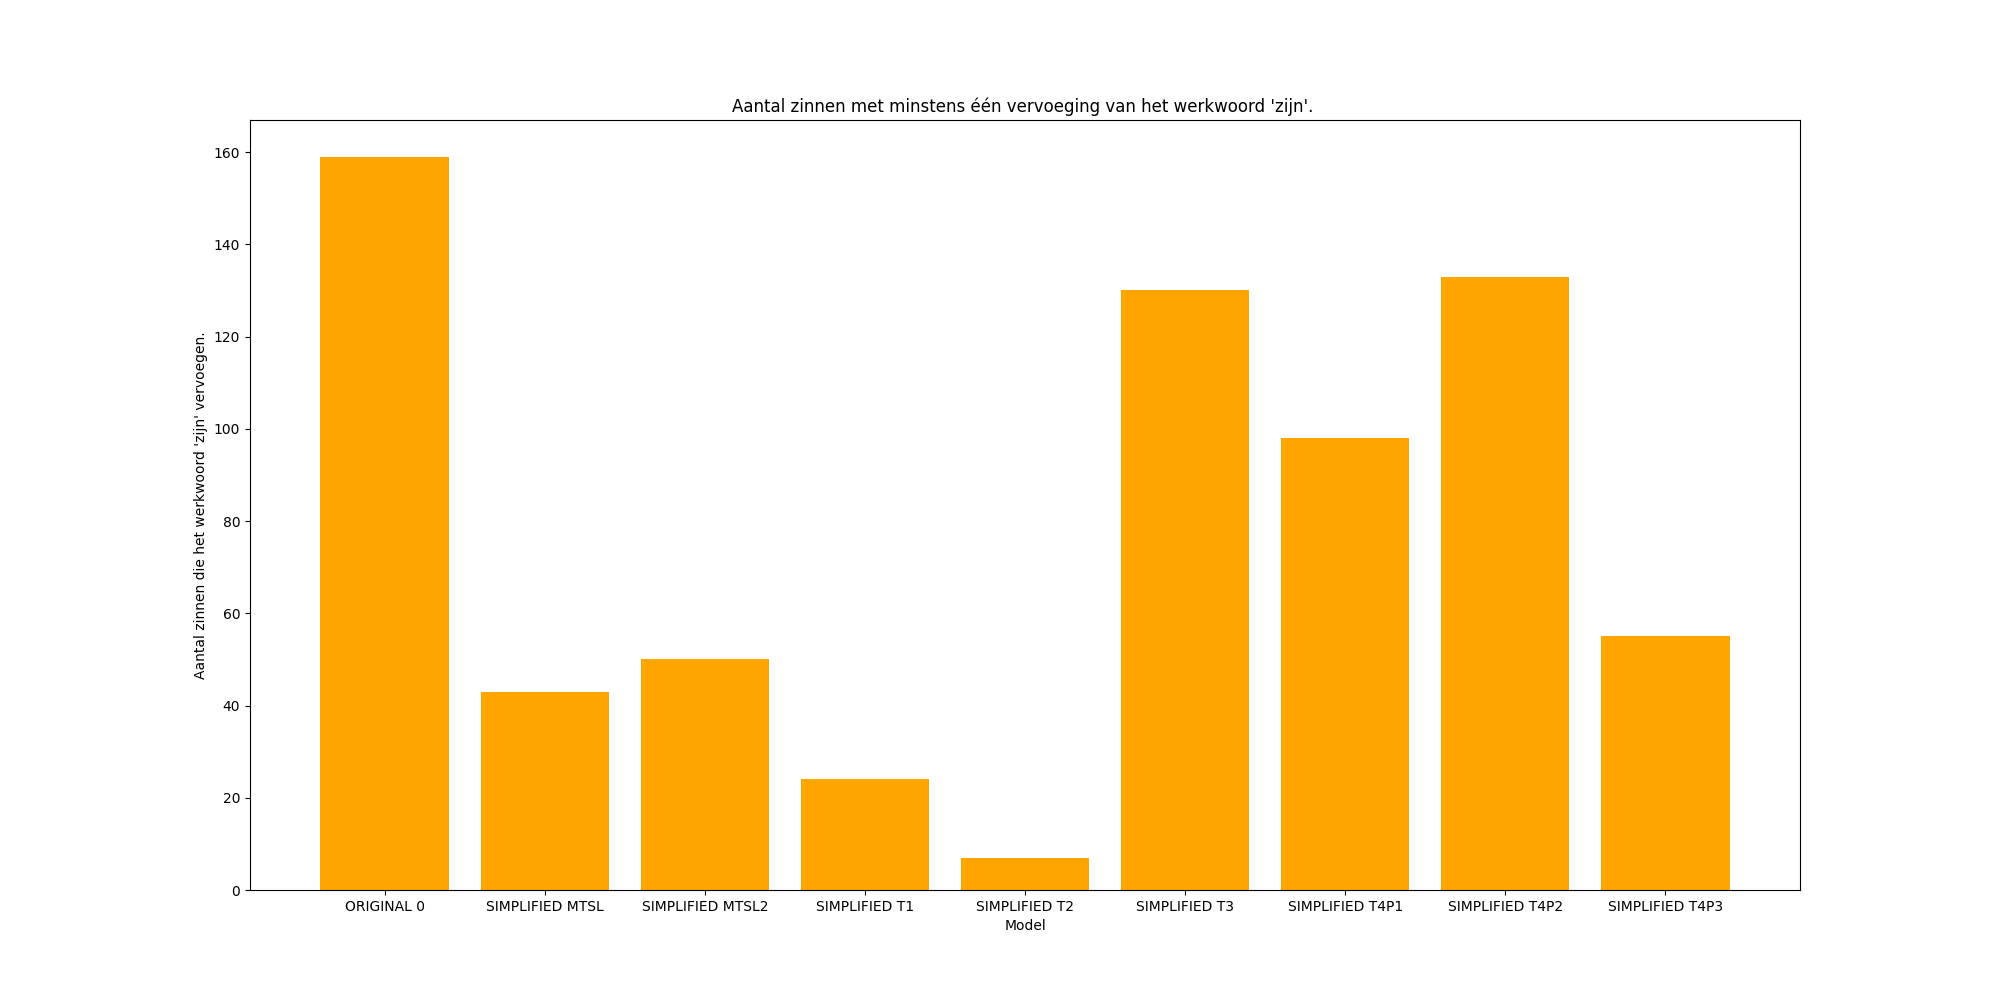
\includegraphics[width=\linewidth]{img/boxplot-tobe-a2.png}
	\caption{Gemiddeld aantal vervoegingen van het werkwoord 'zijn' per zin gegroepeerd op model voor A2.}
	\label{img:histplot-tobe-a2}
\end{figure}


\begin{itemize}
	\item Acroniemen behouden
	\item Inschatting van de doelgroep
	\item Behoud van kern- en bijzaken
	\item Bronvermelding behouden
	\item Formaatwijzigingen
	\item Citeren en parafraseren
\end{itemize}


T4P1 en T4P2 vertalen Engelstalige vaktermen naar het Nederlands. Zo blijft de afkorting voor DPKIA intact, maar vertaalt T4P1 hetzelfde woord naar het Nederlands.  T1, T2, T3 en T4P3 houden hier echter geen rekening mee en behouden de oorspronkelijke versie van de tekst. Bij de handmatige vereenvoudiging schrijft de auteur alle afkortingen voluit, zoals beschreven in de richtlijnen. % GPT heeft geen weet wat deze acroniemen zijn.

\medspace

Alle taalmodellen kunnen lexicale vereenvoudiging toepassen. De handmatig vereenvoudigde referentieteksten bevatten zinnen die vakjargon gebruiken op het niveau van 15 tot 18 jarige studenten. T4P1 kan uitleg tussen ronde haakjes schrijven, wanneer het geen eenvoudiger synoniem kan vinden. T4P1, T1, T2 en T3 passen woorden aan, maar schrijven geen extra uitleg. T4P3 past deze techniek minder toe dan de vooraf vermelde taalmodellen.

\medspace

Geen taalmodel wijkt af van de hoofdgedachte van het oorspronkelijke wetenschappelijk artikel. Hoewel T1, T2 en T3 deels afgebroken zinnen kan genereren, bevatten deze zinnen de hoofdgedachte. Tenslotte verwerken T1, T2 en T3 de APA- en California bronvermeldingen niet in de vereenvoudigde teksten. Hoewel T4 deze wel verwerkt, bevat de tekst na een vereenvoudiging deze bronvermeldingen niet meer. % Het taalmodel verwerkt of herwerkt deze tekst niet.

\medspace

T4P3 maakt de zinnen korter door langere zinnen op te splitsen. T1, T2 en T3 behalen een gelijke zinslengte als dat van de oorspronkelijke zin. T4P1 en T4P2 voegen 

% Taalmodellen T1, T2 en T3 zijn niet in staat om syntactische vereenvoudiging op een tekst toe te passen. Alleen T4 kan via P1, P2 en P3 de zinsyntax verlagen. Hoewel alle geteste taalmodellen in staat zijn om lexicale vereenvoudiging te realiseren, wordt de nauwkeurigheid van de doelgroepsinschatting in twijfel getrokken. De referentieteksten schatten de doelgroep correct in door bekend jargon niet aan te passen, maar wel nieuwe jargon aan te passen als er een beschikbaar synoniem is. Daarnaast kan P1 van T4 ook de coherentie van een meegegeven paragraaf bevorderen, door onder meer omslachtige zinsstructuren aan te passen naar signaalwoorden. 

% T4 heeft verschillende voordelen ten opzichte van T1, T2 en T3 bij gepersonaliseerde ATS voor wetenschappelijke artikelen. Ten eerste kan T4 het aantal zinnen verminderen, terwijl T1, T2 en T3 juist meer zinnen genereren in de vereenvoudigde tekst. T4 slaagt er ook in om gemiddeld minder woorden per zin te gebruiken dan de oorspronkelijke tekst, terwijl de andere modellen dit niet kunnen bereiken. Daarnaast weet T4 langere woorden weg te laten en complexe woorden beter te vervangen dan T1, T2 en T3. Dit resulteert in vereenvoudigde wetenschappelijke artikelen die vergelijkbaar zijn met de referentieteksten. T4 is ook uniek in zijn vermogen om de zinsyntax te verlagen en de coherentie van een paragraaf te verbeteren door signaalwoorden toe te passen. Een ander voordeel van T4 is dat het flexibeler is in het aanpassen van het formaat van de uitvoer. Terwijl T1, T2 en T3 alleen doorlopende tekst produceren, kan T4 ook het formaat wijzigen naar een tabelvorm of opsomming indien expliciet gevraagd. Deze voordelen maken T4 een aantrekkelijke keuze ten opzichte van T1, T2 en T3 bij gepersonaliseerde ATS van wetenschappelijke artikelen voor scholieren met dyslexie in de derde graad van het middelbaar onderwijs.

\section{Het prototype voor tekstvereenvoudiging met ATS vergeleken met top-of-the-line tools.}

% deelvraag: Hoe kan een intuïtieve en lokale webtoepassing worden ontwikkeld die zowel scholieren met dyslexie als docenten helpt bij het vereenvoudigen van wetenschappelijke artikelen met behoud van semantiek, jargon en zinsstructuren?

Vanuit de homepagina kunnen eindgebruikers drie schermen kiezen: het lerarencomponent, het scholierencomponent en een instellingenpagina.

In de instellingenpagina kunnen eindgebruikers de opmaakopties aanpassen naargelang hun keuze. 

\begin{center}
	\begin{figure}[H]
		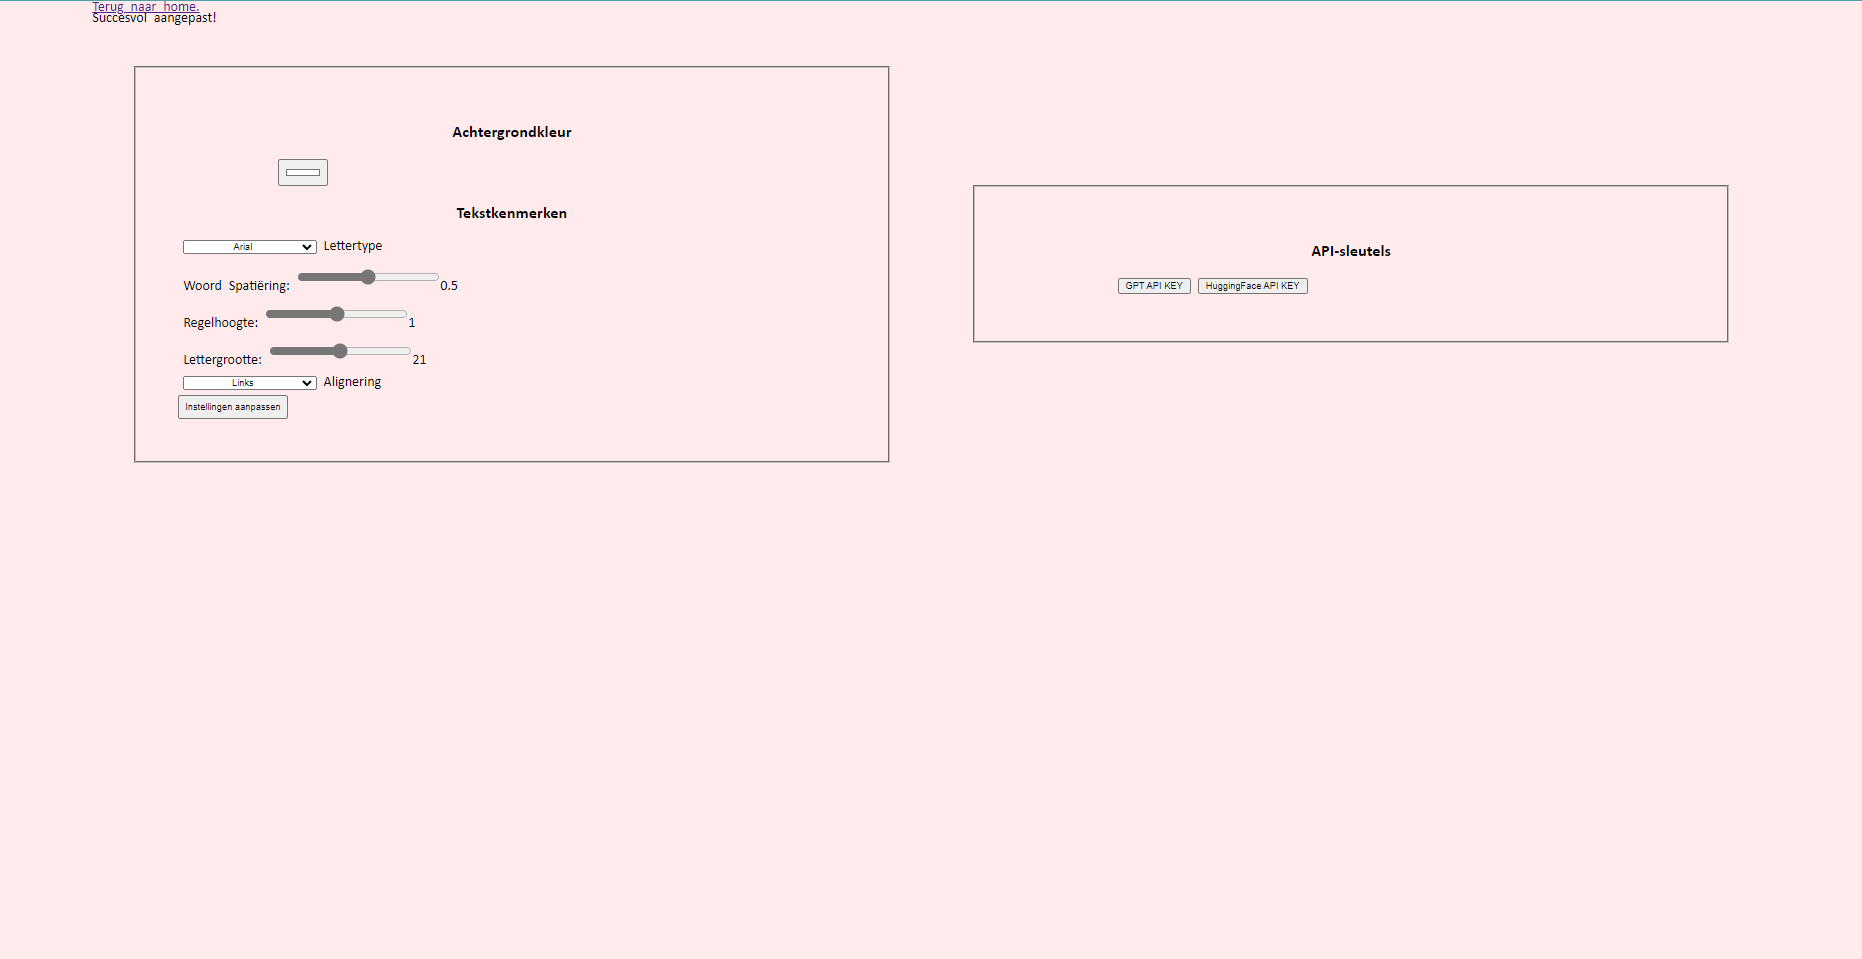
\includegraphics[width=\linewidth]{img/website-instellingen.png}
		\caption{Voorbeeldweergave van de instellingenpagina.}
		\label{img:website-instellingen}
	\end{figure}
\end{center}

Bovendien stelt het prototype gebruikers in staat om op basis van gegeven parameters automatisch personaliseerbare PDF- en Word-documenten te genereren.

\begin{figure}
	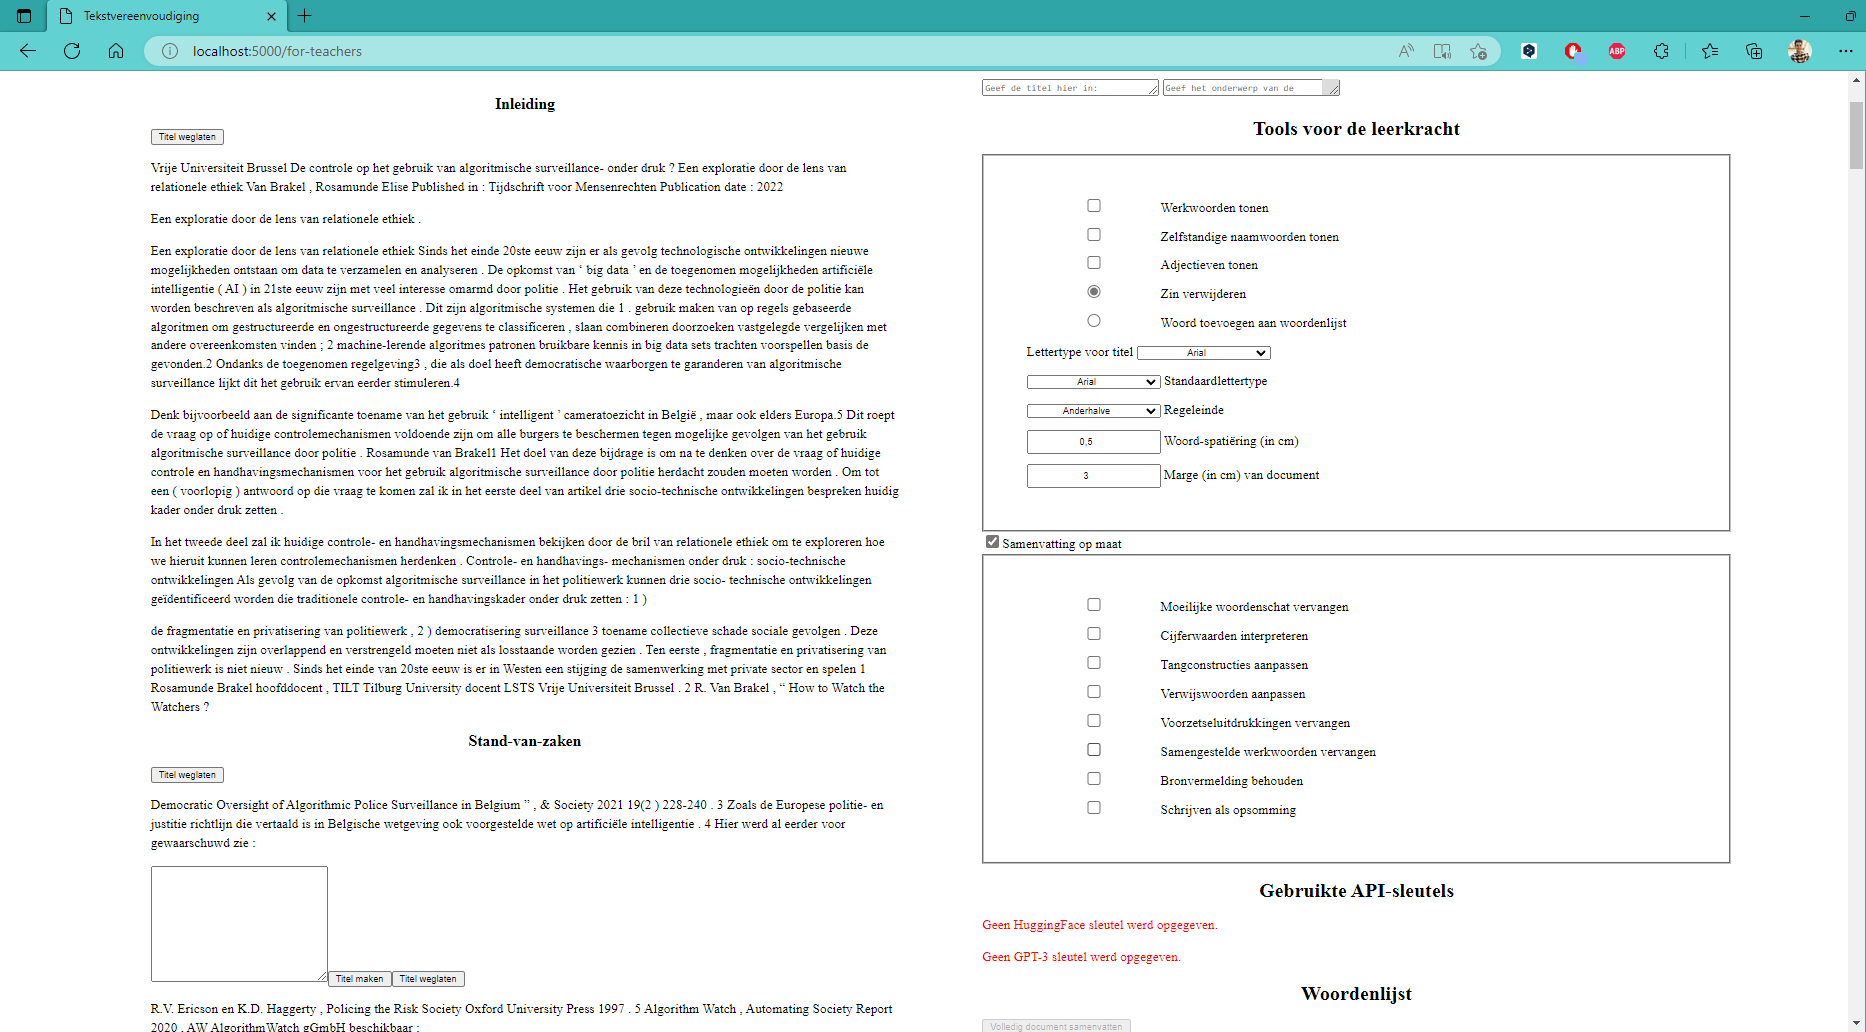
\includegraphics[width=\linewidth]{img/proto-lerarencomponent.png}
	\caption{Een mogelijke weergave van het lerarencomponent met het wetenschappelijk artikel van \textcite{VanBrakel2022} als input.}
	\label{img:proto-lerarencomponent}
\end{figure}

\begin{center}
	\begin{figure}[H]
		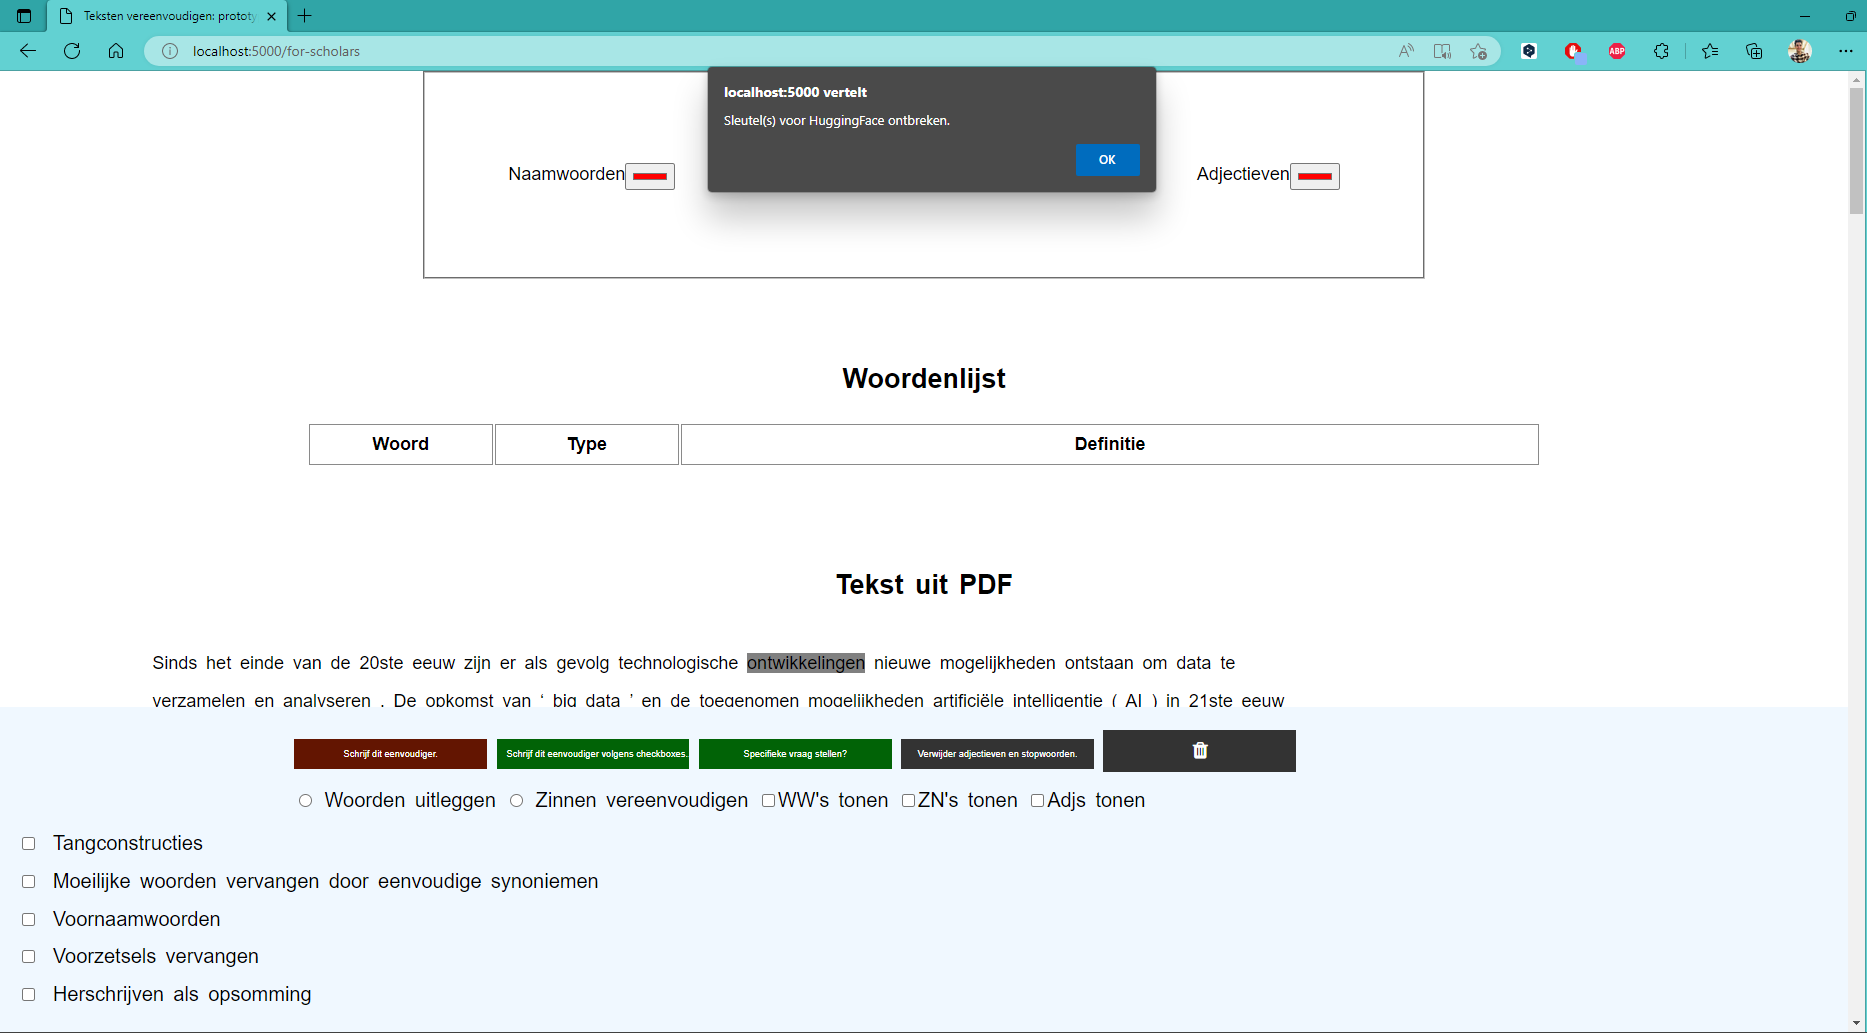
\includegraphics[width=\linewidth]{img/proto-melding.png}
		\caption{Een voorbeeldweergave van het scholierencomponent.}
		\label{img:proto-homescreen-scholieren}
	\end{figure}
\end{center}

Figuur \ref{img:proto-pos-tagging-scholieren} toont een voorbeeldweergave van deze functionaliteit. 

\begin{center}
	\begin{figure}[H]
		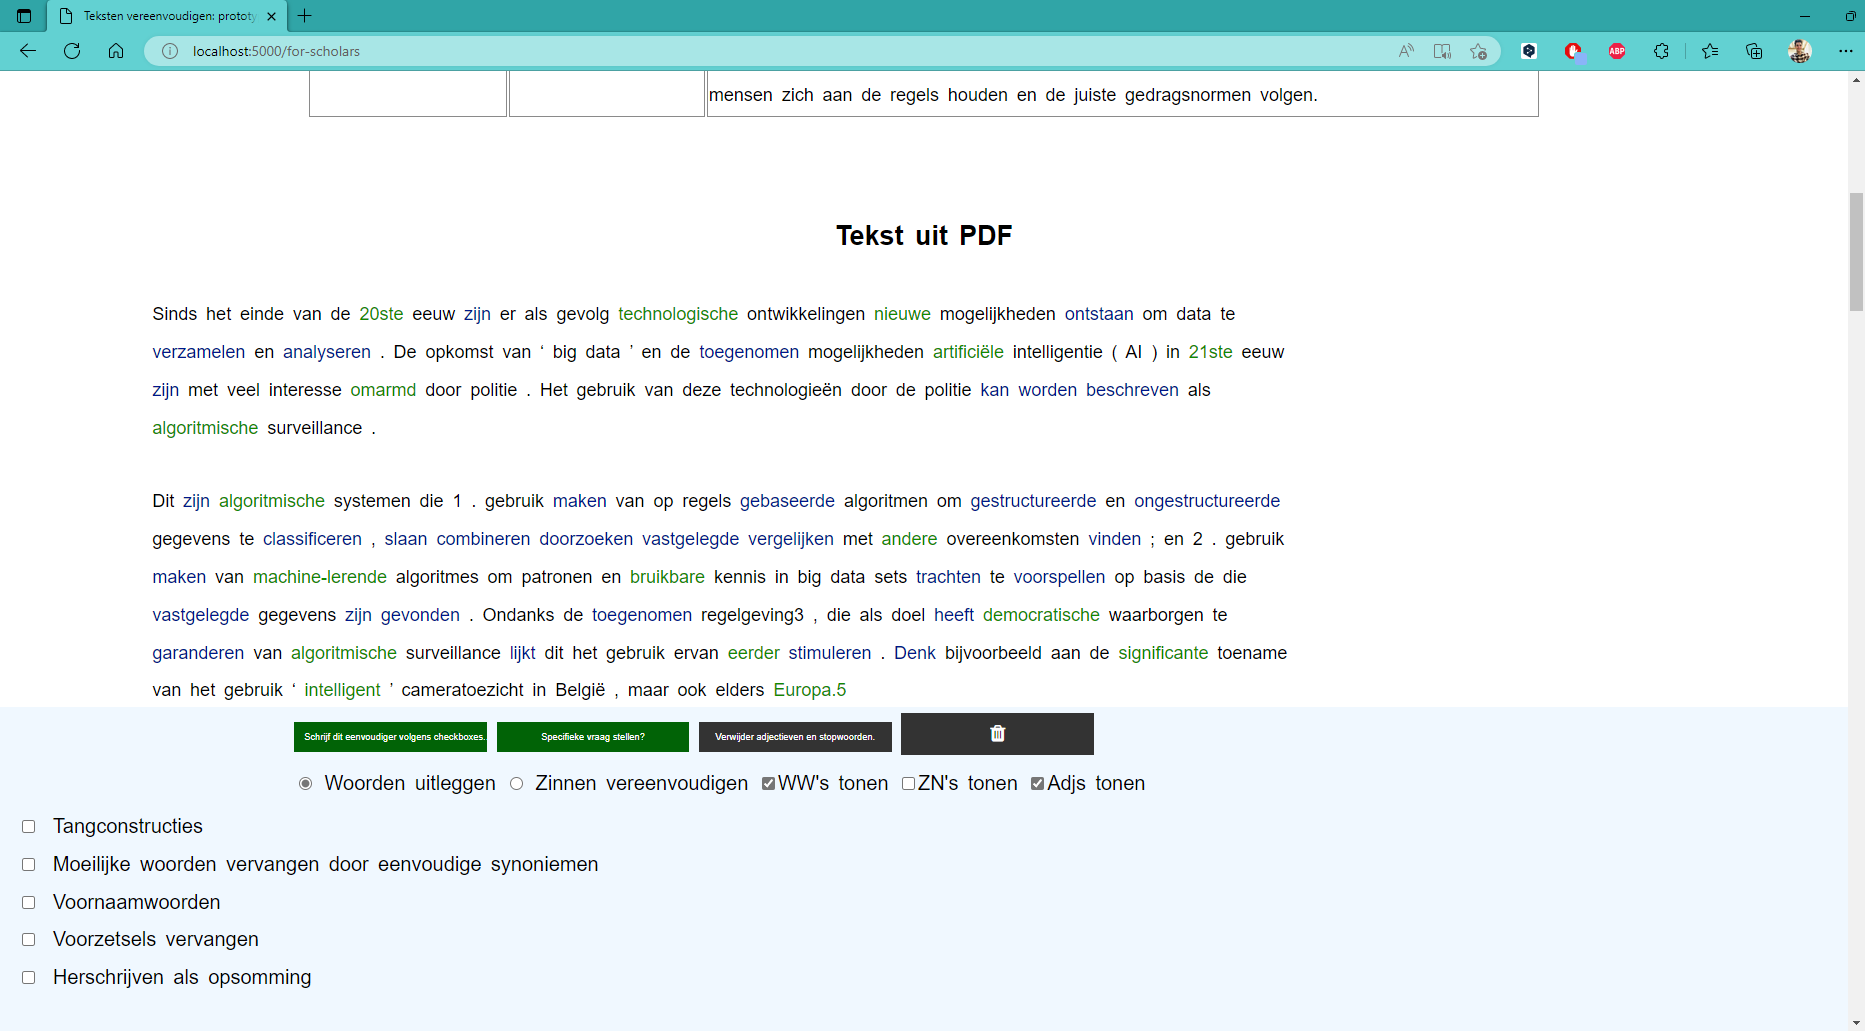
\includegraphics[width=\linewidth]{img/proto-pos-tagging.png}
		\caption{Een voorbeeldweergave van de toepassing van PoS-tagging bij het scholierencomponent.}
		\label{img:proto-pos-tagging-scholieren}
	\end{figure}
\end{center}

\begin{center}
	\begin{figure}[H]
		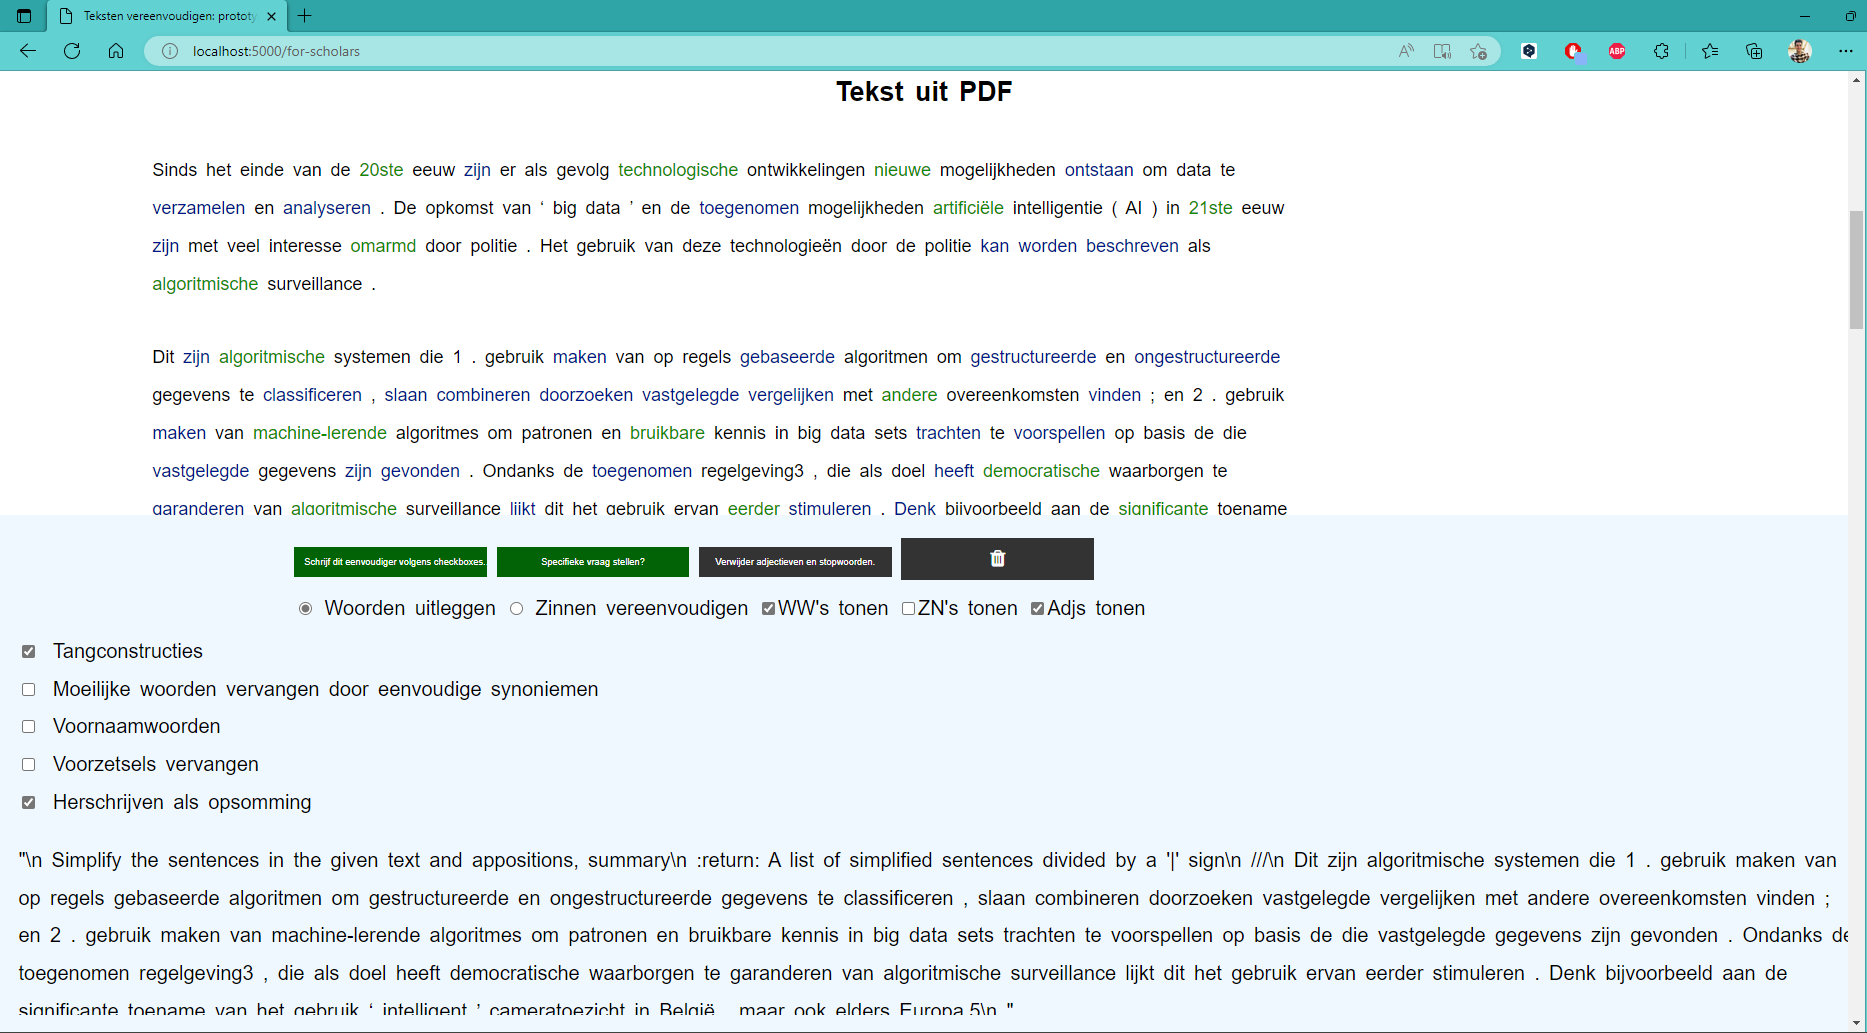
\includegraphics[width=\linewidth]{img/proto-opsomming-1.png}
		\caption{Stap 1 van een gepersonaliseerde tekstvereenvoudiging in het scholierencomponent.}
		\label{img:proto-scholieren-step-1}
	\end{figure}
\end{center}

\begin{center}
	\begin{figure}[H]
		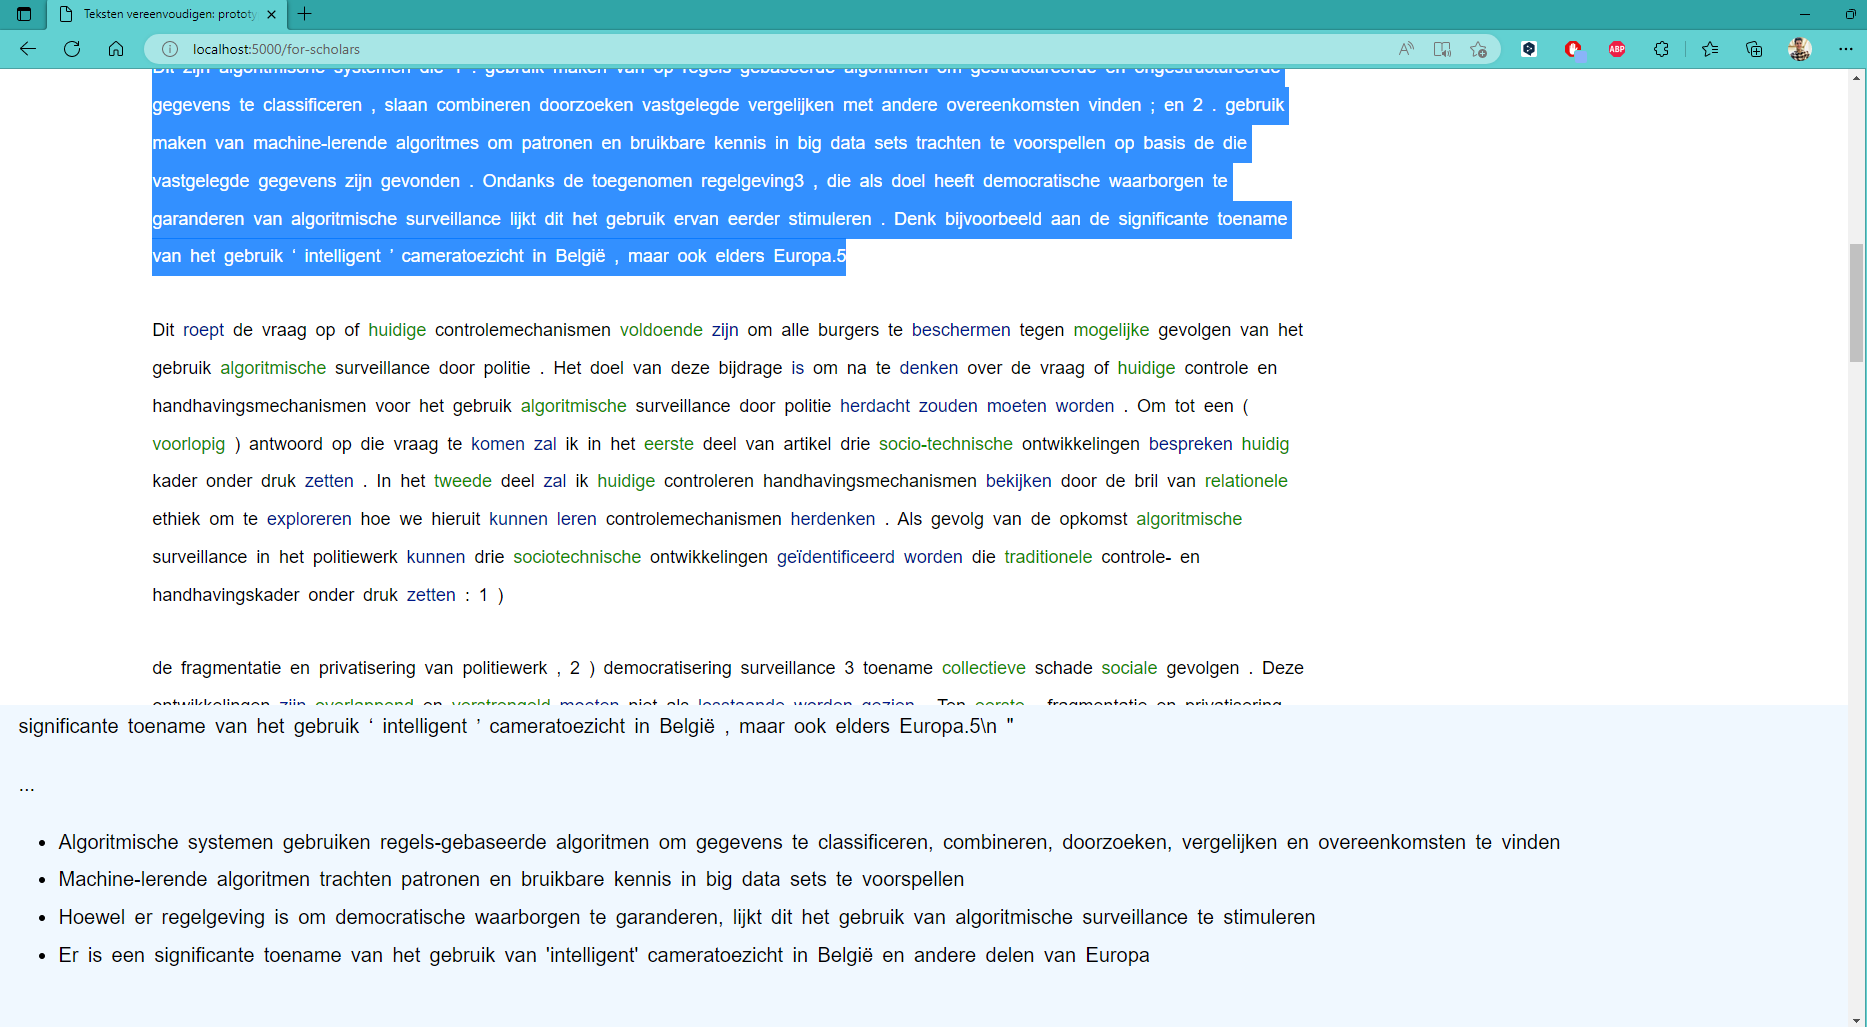
\includegraphics[width=\linewidth]{img/proto-opsomming-3.png}
		\caption{Stap 3 van een gepersonaliseerde tekstvereenvoudiging in het scholierencomponent.}
		\label{img:proto-scholieren-step-3}
	\end{figure}
\end{center}

Het scholierencomponent biedt functionaliteiten aan om een ondersteunende ervaring aan scholieren toe te lenen. Zo kunnen scholieren specifieke zinnen vereenvoudigen door middel van gepersonaliseerde ATS. Figuren \ref{img:step-1-proto-vraagstelling} en \ref{img:step-2-proto-vraagstelling} tonen een tweede functionaliteit. Zo kunnen scholieren specifieke vragen stellen aan het prototype door middel van een gecentreerd invoerscherm.

\begin{center}
	\begin{figure}
		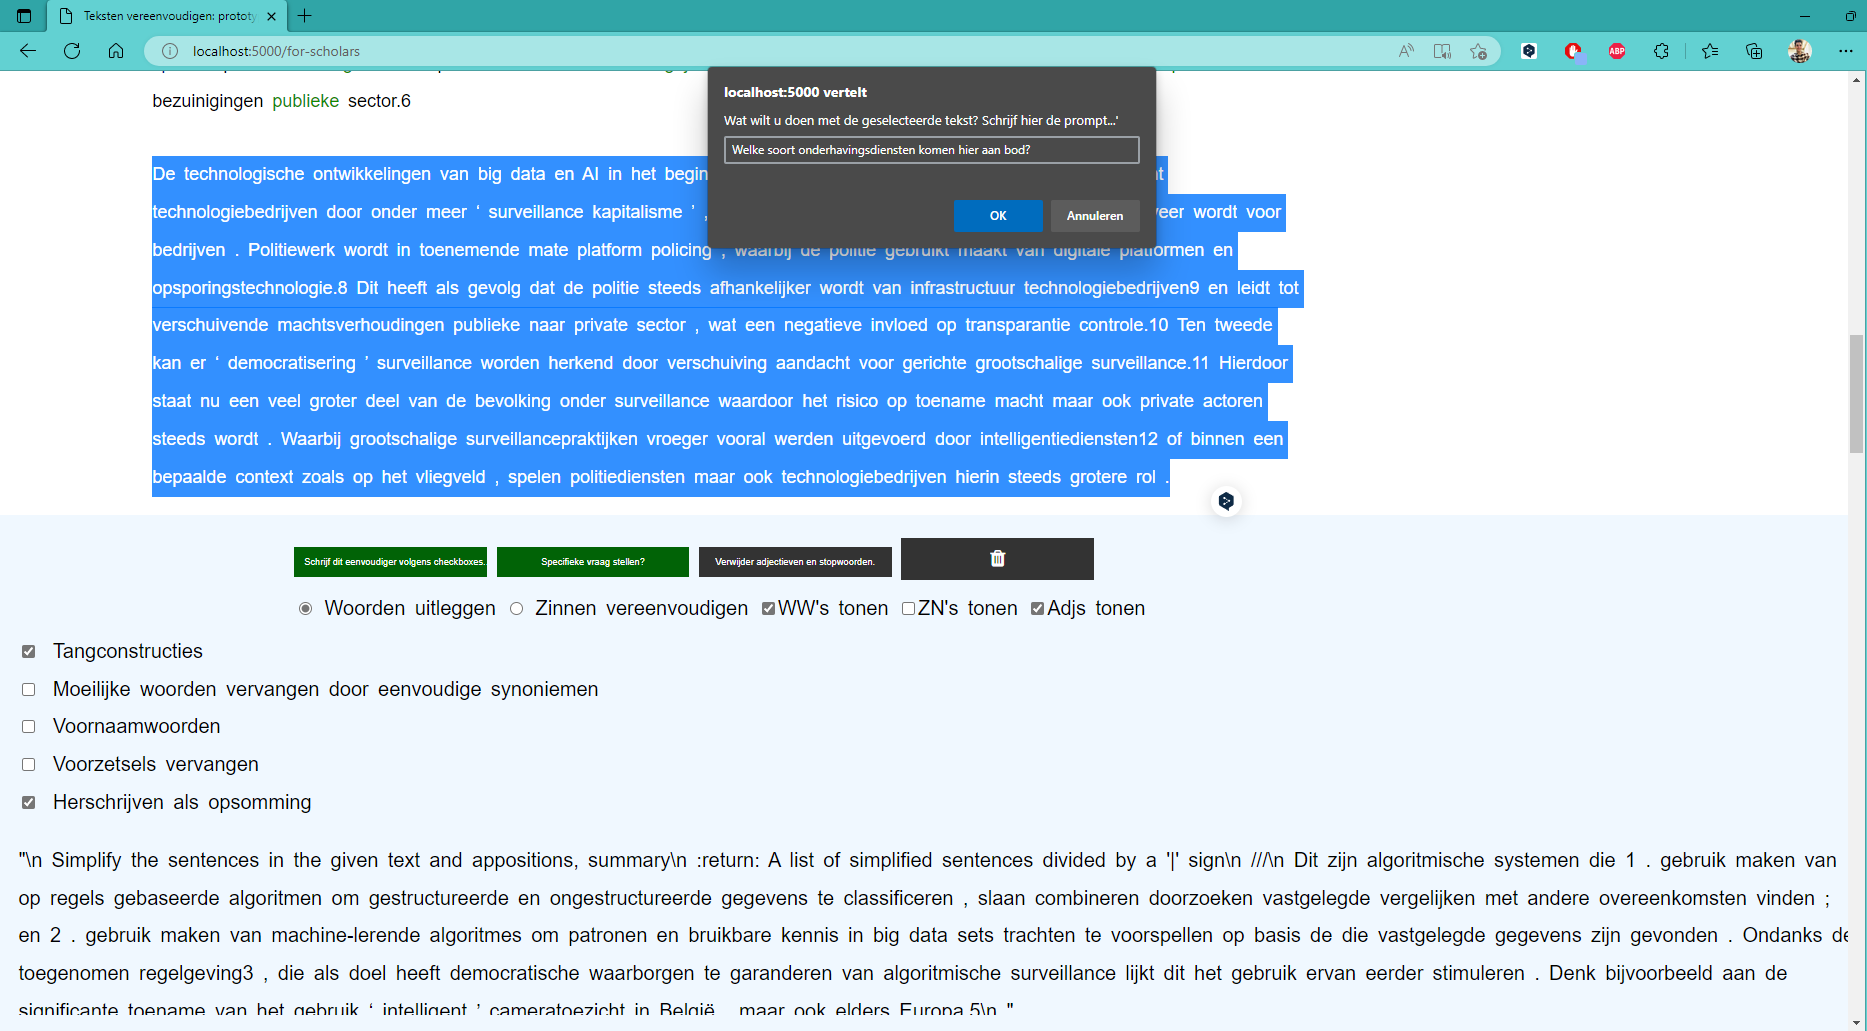
\includegraphics[width=\linewidth]{img/proto-vraagstelling-1.png}
		\caption{Stap 1 bij het stellen van een specifieke vraag bij gemarkeerde tekst.}
		\label{img:step-1-proto-vraagstelling}
	\end{figure}
\end{center}

\begin{center}
	\begin{figure}
		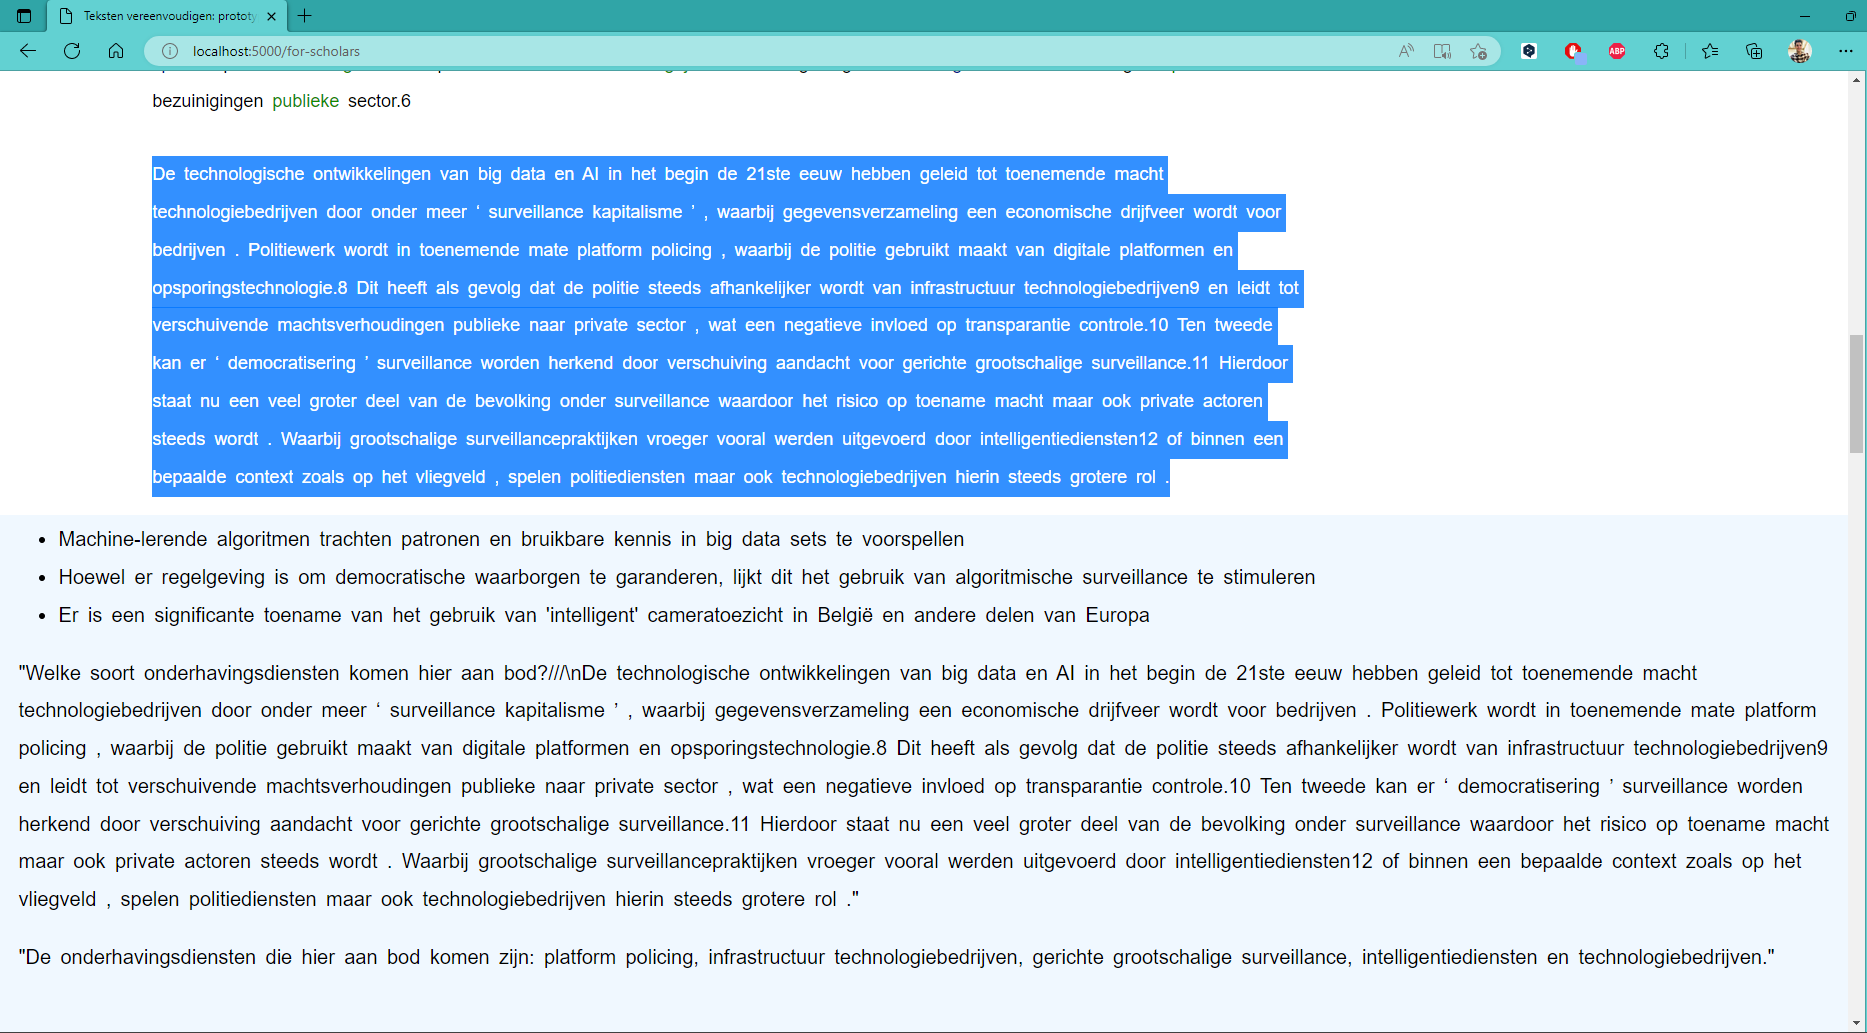
\includegraphics[width=\linewidth]{img/proto-vraagstelling-2.png}
		\caption{Stap 2 bij het stellen van een specifieke vraag bij gemarkeerde tekst.}
		\label{img:step-2-proto-vraagstelling}
	\end{figure}
\end{center}

De ontwikkeling van een prototype voor een gepersonaliseerde ATS van wetenschappelijke artikelen heeft tot doel om ontwikkelaars inzicht te verschaffen in de mogelijkheden om een coherente en lokale webtoepassing te ontwikkelen. Na evaluatie blijkt het prototype te voldoen aan de gespecificeerde functionaliteiten zoals vastgesteld in het Moscow-schema of tabel \ref{img:moscow-table}. Hiermee overtreft het prototype alle andere geteste tools in tabel \ref{table:overview-tools} op alle fronten. Eerdere belemmeringen, zoals het wijzigen van het formaat, waren enkel mogelijk via de commandline of via een chatbot. Het huidige prototype heeft echter intuïtieve handelingen geïmplementeerd om deze obstakels te overwinnen. 

Het prototype bevat functionaliteiten waarmee eindgebruikers wetenschappelijke artikelen kunnen inladen. Daarna krijgen zowel de leraren als de scholieren de mogelijkheid om de tekst te manipuleren door middel van gepersonaliseerde ATS. Zo bevat het prototype alle must-haves uit het moscow-schema. Daarnaast bevat het prototype geen enkele wont-have.

Deze functionaliteiten zijn vergelijkbaar met andere geteste tools in de requirementsanalyse, maar gaan verder dan wat momenteel beschikbaar is in chatbots die geavanceerde logica gebruiken voor gepersonaliseerde ATS. Zowel scholieren als docenten kunnen ook de opmaakopties van de toepassing aanpassen aan hun persoonlijke voorkeuren bij het lezen van wetenschappelijke artikelen. 

% Dit wordt gerealiseerd door woordenlijsten te reproduceren na een zorgvuldige handmatige selectie van moeilijke woorden. Het prototype is lokaal op te zetten met behulp van Docker, hoewel voor het gebruik ervan een internetverbinding vereist is, net als bij andere tools in tabel \ref{table:overview-tools}.